
\chapter[Expanding the atlas of human disease variants]{Expanding the atlas of variant effects in human disease genes}
\label{ch:data2}

As in the previous chapter, the work described here is the result of a team effort including multiple members of the Roth Lab as well as other collaborators. Wet lab procedures were executed by Marta Verby, Song Sun, Atina Co\'te and Jennifer Knapp, while computational aspects of the work were developed and implemented by myself, except where indicated otherwise.

\section{Introduction}

Within coming decades, millions of people will have their genome sequenced. Unfortunately, we have limited ability to interpret personal genomes, each carrying 100-400 rare missense variants~\cite{the_1000_genomes_project_consortium_global_2015} of which many must currently be classified as Variants of Uncertain Significance (VUS). For example, gene panel sequencing aimed at identifying germline cancer risk variants in families yielded VUS for the majority of missense variants~\cite{maxwell_evaluation_2016}. While functional variants can be predicted via computational tools such as PolyPhen-2~\cite{adzhubei_predicting_2001} and PROVEAN~\cite{choi_predicting_2012}, these methods can confidently detect only one third as many disease variants as are detectable by experimental assays~\cite{sun_extended_2016}. Unfortunately, experimental assays are either unavailable or economically inviable for most human disease genes. 

Recent DMS studies have provided individual maps for the critical RING domain of BRCA1~\cite{starita_massively_2015} associated with breast cancer risk, and the PPAR$\gamma$ protein associated with Mendelian lipodystrophy and increased risk of type 2 diabetes~\cite{majithia_prospective_2016}. Such maps can not only identify functionality of a clinical variant accurately, but also potentially do so in advance of that variant's first clinical presentation. 

In the previous chapter, a framework for comprehensive high-quality screening of functional effects across all possible missense mutations in human genes was established. The functional complementation assay used in the assay allows for the generation of maps that not only represent the overall functional consequences of mutations, but also serves as a common basis to make maps more directly comparable. In addition, the statistical analysis and machine learning component introduced allows for high overall map quality and completeness. Using this framework a complete functional map for the SUMO E2 conjugase \gene{UBE2I} was created. Here I describe the creation of a map of a second member of the Sumoylation pathway, \gene{SUMO1}. I examine both map in detail before discussing the interpretation of yeast complementation phenotypes in terms of humans. 

To demonstrate the value of the DMS framework in terms of clinical interpretation of variants, a diverse set of six new disease gene maps was added to the atlas: \gene{TPK1} encoding Thiamin Pyrophosphokinase 1, \gene{NCS1} encoding Neuronal Calcium Sensor 1, as well as the paralogues \gene{CALM1}, \gene{CALM2} and \gene{CALM3}, which each encode the protein Calmodulin. The maps are evaluated in terms of pathogenicity prediction and VUS reclassification.

\section{Results}

% \todo{Outline the structure of the results section}

\subsection{A functional map of SUMO E2 recapitulates known biology and poses new questions}

% \todo{Quickly recap how maps for UBE2I and SUMO1 were made}

The DMS map of \gene{UBE2I} produced in the previous chapter paints a comprehensive picture of variant effects on protein function. The complete, refined functional map of UBE2I after imputation and regularization can be seen in Figure~\ref{fig:ube2i-map}. For comparison, additional tracks showing position-specific evolutionary conservation, secondary  structure, relative solvent accessibility and burial in protein-protein interaction interfaces are also shown.  
Based on the map, several observations can be made. Consistent with the results of smaller-scale biochemical studies of the SUMO E2 conjugase\cite{bencsath_identification_2002,bernier-villamor_structural_2002}, the areas most sensitive to mutation are those proximal to the active site (particularly residues 81-88, 90, 92-96, and 127-130), and the N-terminal $\alpha$-helix which mediates four protein interactions including the critical interaction with the E1 SUMO-activating complex. Within the active site, particularly strong sensitivity to mutation can be observed at the cysteine residue at position 93. This is consistent with its central role in E2 function, as it forms a thioester bond with the SUMO C-terminus~\cite{bernier-villamor_structural_2002}.

\begin{landscape}
\begin{figure}[h]
	\centering
	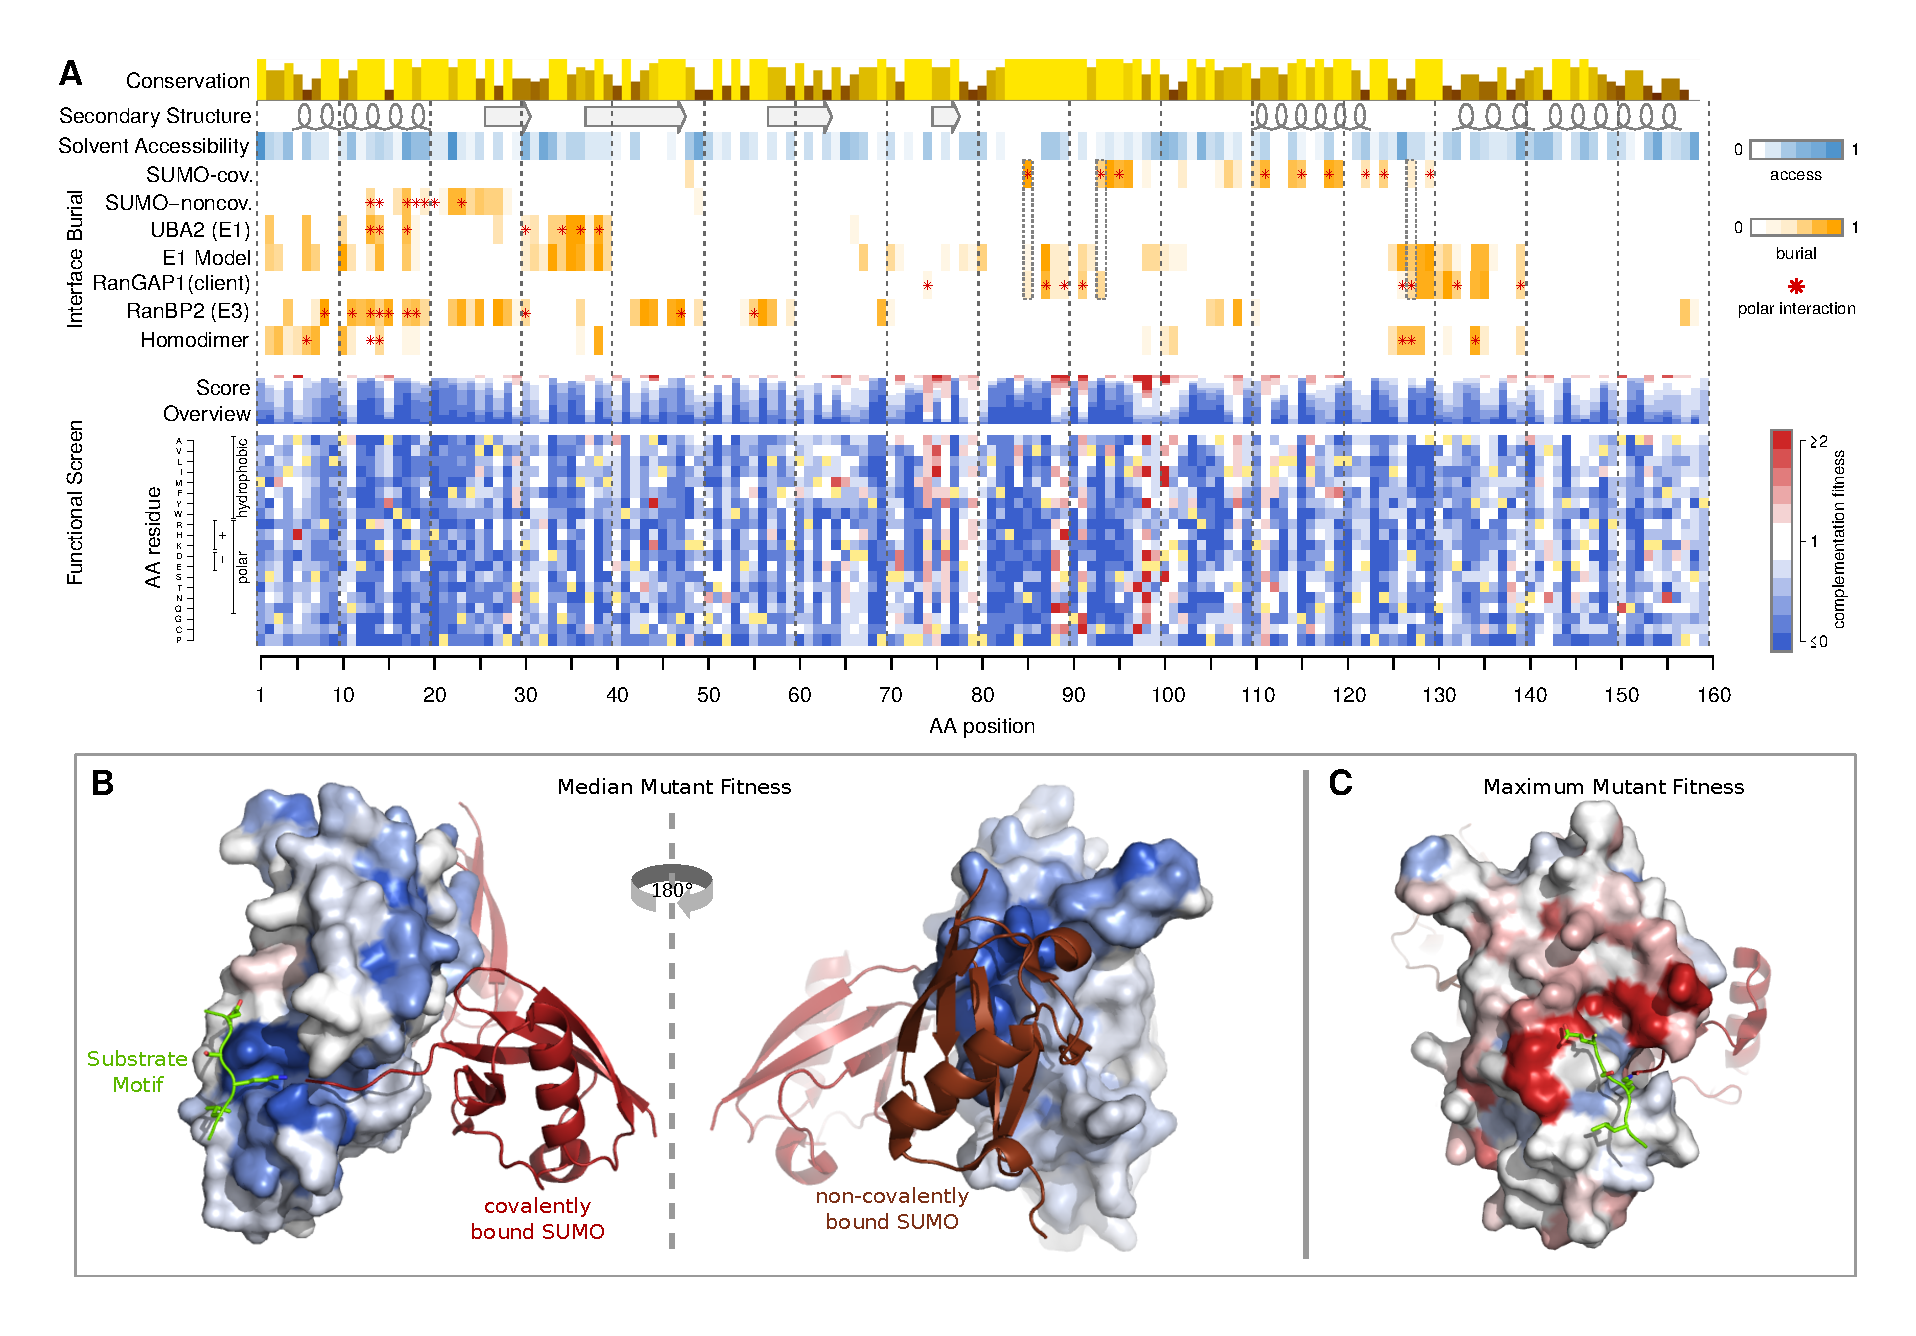
\includegraphics[width=9in]{img/ube2i_map.pdf}
	\caption{Functional map of UBE2I. From top to bottom: Position-wise evolutionary conservation (AMAS); Secondary structure; Relative solvent accessibility; Relative burial in protein-protein interaction interfaces with covalently bound SUMO, non-covalently bound SUMO, the SUMO E1 complex at two different stages of activation, the sumoylation substrate RanGAP1, the E3 RanBP2, and the UBE2I homodimer; A summary track showing the relative number of amino acid changes resulting in different fitness effects; and finally the individual amino acid change effects sorted by physicochemical groups.}
	\label{fig:ube2i-map}
\end{figure}
\end{landscape}

An interesting feature of the map is the alternating tendency towards damaging and benign substitutions across positions 55-65. A comparison with solvent accessibility reveals this to be caused by alternating externally and internally-oriented residues, with the latter positions constrained to be hydrophobic. This alternating tendency is also reflected in evolutionary conservation across these positions. 


All protein-protein interaction interfaces previously captured in co-crystal structures show increased sensitivity to mutation when compared to other surface residues (Figure~\ref{fig:ube2i_interfaces}). When comparing individual protein interaction interfaces, the most substantial fitness defects are observed in those for the E1 activating complex binding interface and the covalent and non-covalent SUMO binding interfaces (Figure~\ref{fig:ube2i_interfaces}A). While the homodimerization interface also shows significant sensitivity (Wilcoxon $P=6.87\cdot 10^{-21}$), the effects are not as severe as those at the E1 interface (Wilcoxon $P=4.28\cdot 10^{-8}$) (Figure~\ref{fig:ube2i_interfaces}B). This is consistent with the Alontaga and colleagues' hypothesis regarding its involvement in SUMO chaining~\cite{alontaga_rwd_2015}, as in yeast SUMO chain formation has so far only been observed to be involved in meiosis~\cite{cheng_sumo_2006}, which is not a mechanism vital to fitness in a complementation assay. Alontaga \etal\ also postulate however, that non-covalent SUMO binding is necessary for SUMO chain formation. In contrast to the homodimerization interface, the non-covalent SUMO binding interface shows a much stronger sensitivity to mutation (Wilcoxon $P=4.73\cdot 10^{-8}$). This may be due to two different reasons: (i) there is a 27\% overlap between the interface for non-covalent SUMO binding interface and the interface for E1-E2 binding, which is among the most sensitive surfaces of UBE2I; and (ii) non-covalent SUMO binding also plays an important role as an adapter for many E3 proteins~\cite{cappadocia_structural_2015}.


\begin{figure}[h!]
	\centering
	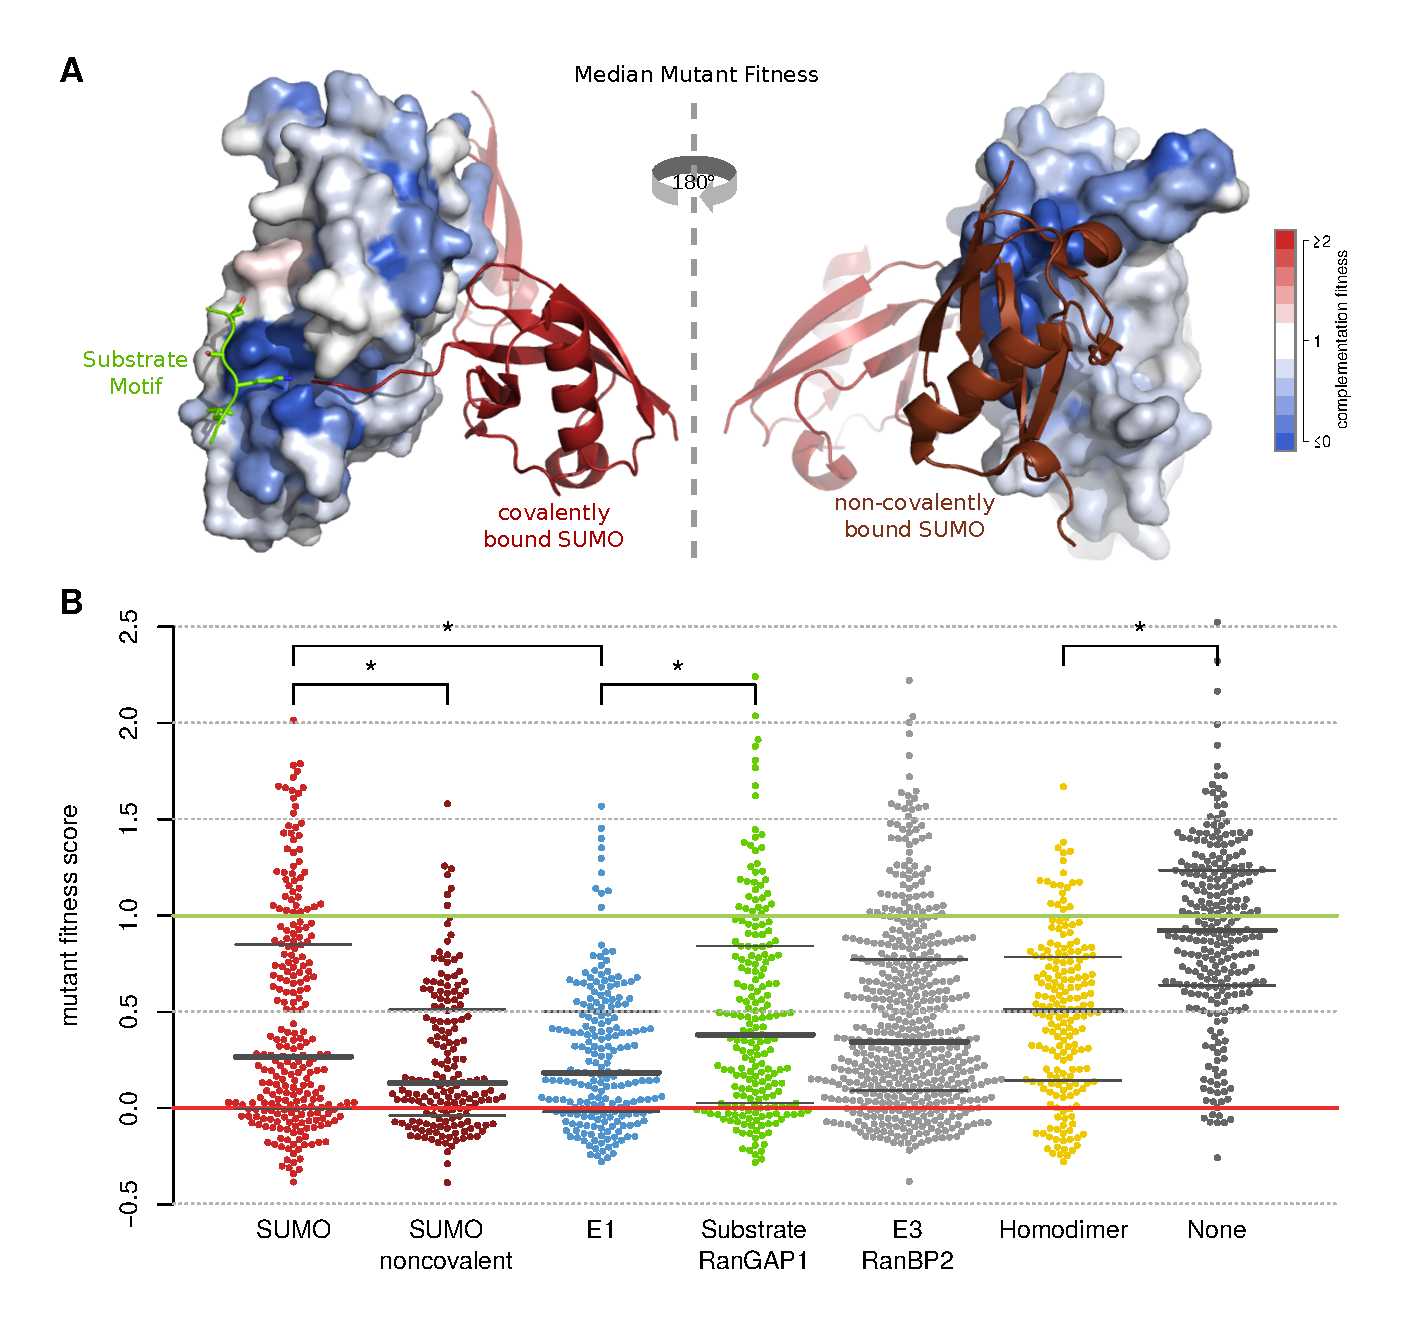
\includegraphics[width=\textwidth]{img/ube2i_interfaces.pdf}
	\caption{Complementation fitness of mutations at interaction interfaces. A) Median mutant fitness mapped to the crystal structure of UBE2I. The $\Psi$KxE substrate recognition motif is shown as green stick model, covalently and non-covalently bound SUMO are shown as crimson and brown cartoon model, respectively. B) Mutant fitness scores distributions for residues at different interaction interfaces (and non-interface surfaces as control). P-values from one-sided Wilcoxon tests. Bold bars represent medians, thin bars indicate 25\% and 75\% quartiles.}
	\label{fig:ube2i_interfaces}
\end{figure}

Another interesting observation can be made with respect to a known phosphorylation site on the surface of UBE2I. Su and colleagues previously discovered that phosphorylation of Serine 71 via the Cyclin-dependent Kinase CDK1 results in sumoylation hyperactivity~\cite{su_phosphorylation_2012}. The map shows that substitutions with phosphomimetic residues at this position lead to hyperactive complementation, consistent with Su~\etal's observations. Furthermore, other residues amenable to phosphorylation are also tolerated, while hydrophobic replacements are generally deleterious (Figure~\ref{fig:phosphosite}).


\begin{figure}
	\centering
	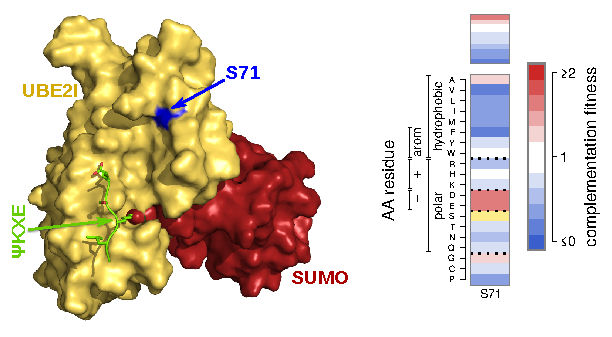
\includegraphics[width=\textwidth]{img/phosphosite.pdf}
	\caption{Phosphorylation site of UBE2I shows hyperactive complementation when mutated to phosphomimetic residues.}
	\label{fig:phosphosite}
\end{figure}


\subsubsection{Substrate specificity shifts and E2 hyperactivity}
\label{sec:hypercomp}
Intriguingly, many sites show fitness that is better than wildtype (e.g., positions 74, 76, 88, 89, 91 and 98). Manual functional complementation spotting assays confirmed that complementation with these mutants allows greater growth than does the wild type human protein, but resemble more closely the growth at the permissive temperature for the \textit{ubc9-ts} strain (Figure~\ref{fig:hyperactive}A). One might be tempted to interpret these cases as reversions to residues present in the yeast protein. However, a comparison of fitness score distributions between changes to \species{S. cerevisiae}  residues and those occurring in the distant species \species{Dictyostelium~discoideum} (amoeba) or \species{Drosophila~melanogaster} (fly) showed no significant difference (Figure~\ref{fig:hyperactive}B). Recognizing that in this assay, human UBE2I must function with the yeast versions of other sumoylation pathway members, it stands to reason that some substitutions could be adaptive by improving compatibility with yeast interaction partners. A comparison with co-crystal structure data~\cite{gareau_determinants_2012} shows that many of the hypercomplementing residues are located on the surface facing the general direction of the substrate, with some being in direct contact with the substrate's sumoylation motif (Figure~\ref{fig:hyperactive}C). This suggests a possible adaptation via improved recognition of substrates for which sumoylation is most important for yeast growth. Indeed, \textit{in vitro} sumoylation assays performed previously for a small number of UBE2I mutants revealed increased sumoylation for some substrates~\cite{bernier-villamor_structural_2002}. Comparing the map with these sumoylation assay results, I observed many cases of substrate specificity shift (Figure~\ref{fig:hyperactive}D). Of the three cases tested in the sumoylation assay that showed hyperactive behaviour in the map (E98A, T91A and K74A), one displayed hyperactive sumoylation of P53, while two displayed decreased sumoylation of P53 and I$\kappa$B$\alpha$. However, similar behaviour was seen for 3 other variants (D100, P128A and S89A), which scored as wildtype-like in the map. Most cases for which P53 saw wild-type level sumoylation showed either wildtype-like or slightly below complementation in the map. Finally, the four cases that disrupted sumoylation of all substrates were strongly deleterious in the map. In conclusion, variants that either positively or negatively or negatively affect P53 sumoylation levels \textit{in vitro} appear show either wildtype-like or hyperactive complementation in yeast. This may indicate that differential sumoylation of one or more yeast proteins with a P53-like interface positively affects yeast growth.


\begin{figure}[h!]
	\centering
	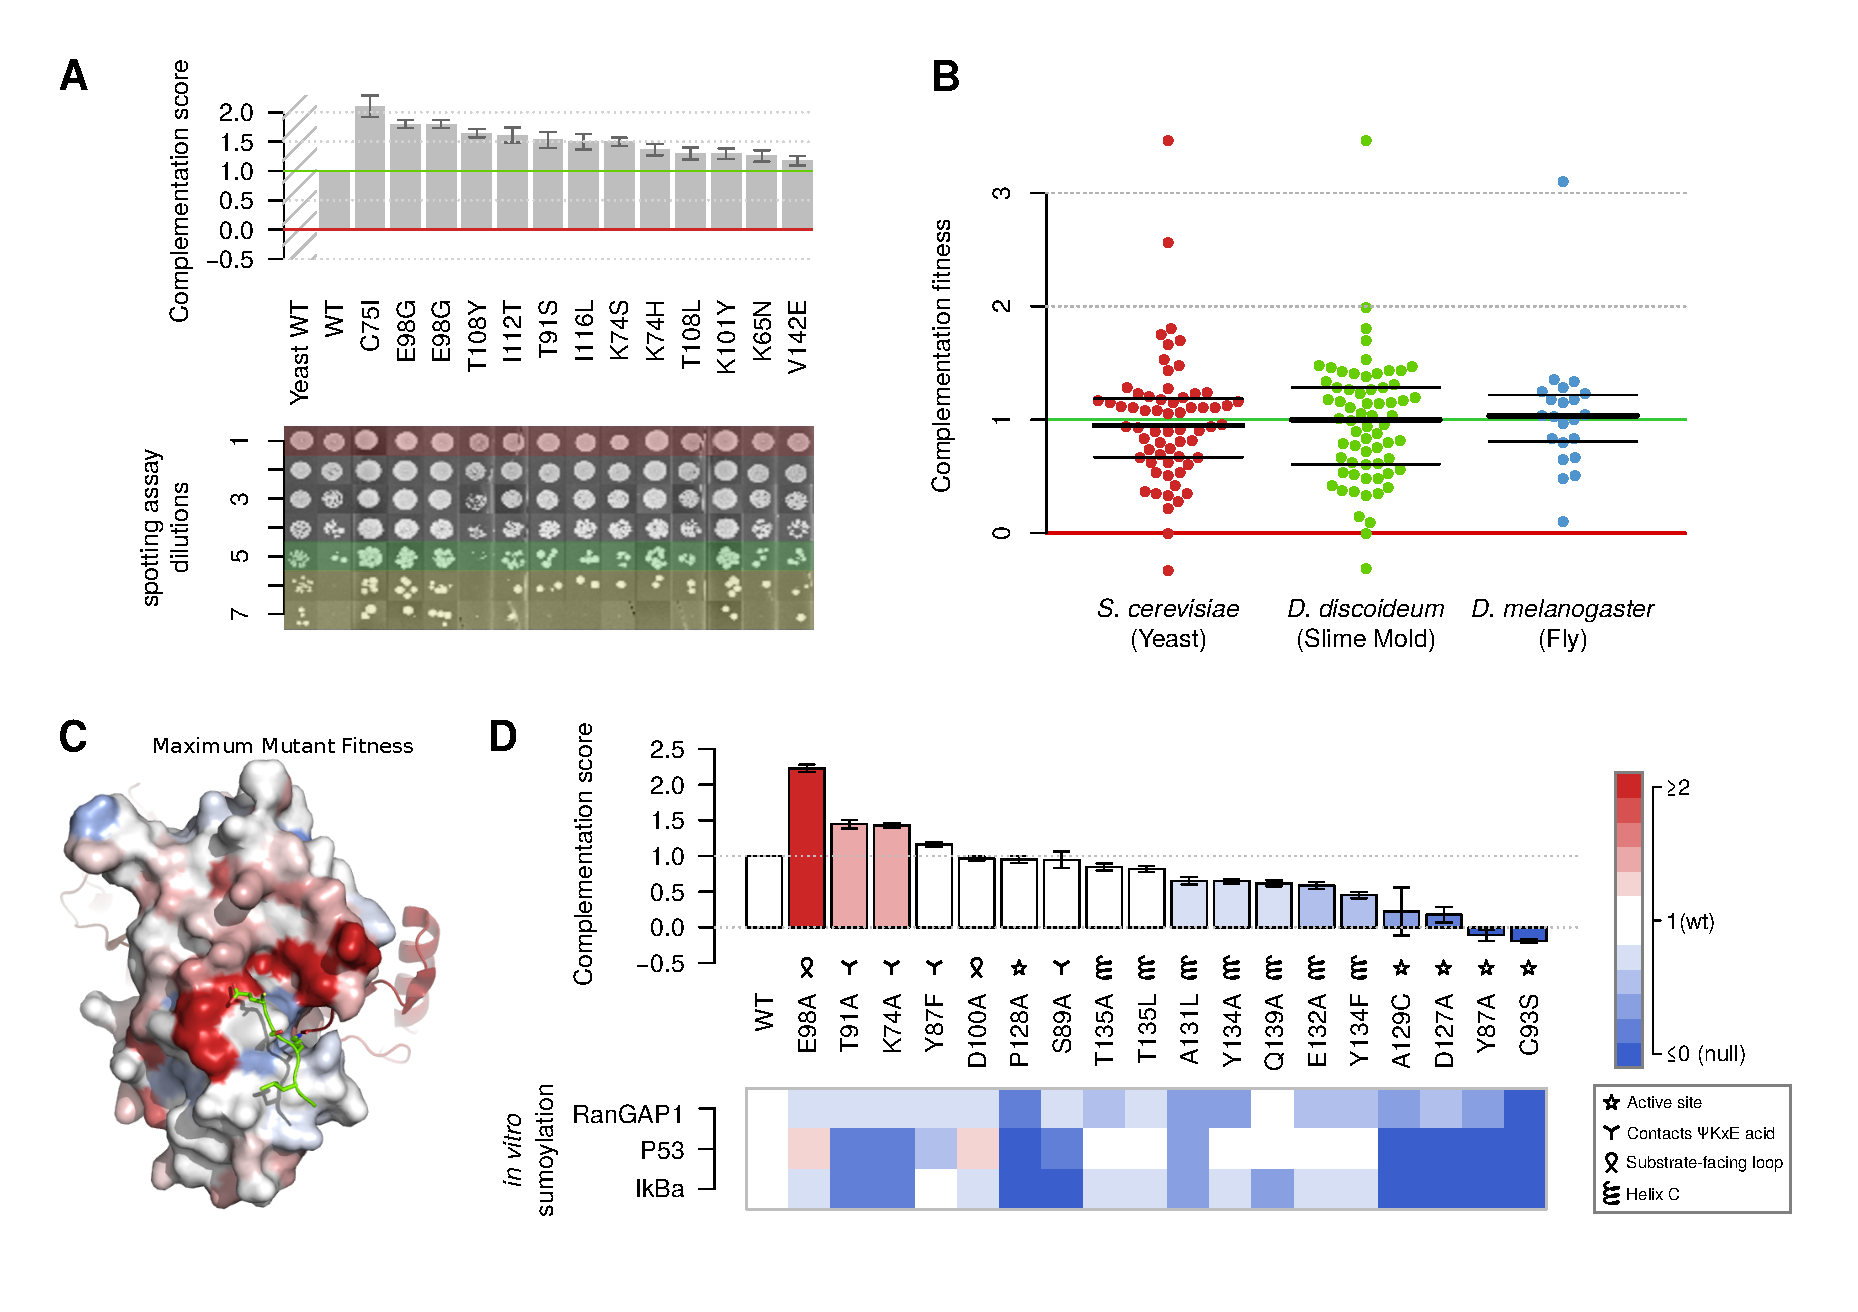
\includegraphics[width=\textwidth]{img/hyperactive.pdf}
	\caption{Hyperactive complementation in UBE2I. A) Variants scoring higher than the wildtype controls show stronger growth in manual complementation spotting assays and resemble the WT yeast. B) Distribution of scores for changes to residues naturally occurring in yeast, amoeba and fly are not significantly different from each other. C) Maximum mutant score mapped to amino acid positions on UBE2I structure. Hyperactive mutations are clustered at the substrate recognition site. Structure data from \texttt{PDB:3UIP}~\cite{gareau_determinants_2012} D) \textit{In vitro} sumoylation assay data from Bernier-Villamor~\etal~\cite{bernier-villamor_structural_2002} in comparison to the complementation fitness scores.}
	\label{fig:hyperactive}
\end{figure}


As Figure~\ref{fig:hyperactive}D shows, substrate specificity does not paint a complete picture of the mechanisms potentially underlying hyperactive complementation. A particularly interesting exception can be observed at residues A15 and T108. Both residues harbor hyperactive mutations but do not face towards the substrate. Instead, they form part of the interface with the E3 SUMO ligase RanBP2, and flank a small cavity on UBE2I's surface into which RanBP2 inserts a phenylalanine residue upon binding~\cite{gareau_determinants_2012}. Changing either A15 or T108 into aromatic residues results in a large fitness increase (Figure~\ref{fig:pi-stack}). This may be the result from the emergence of a $\pi$-stack interaction that strengthens E2-E3 binding.

\begin{figure}[h!]
	\centering
	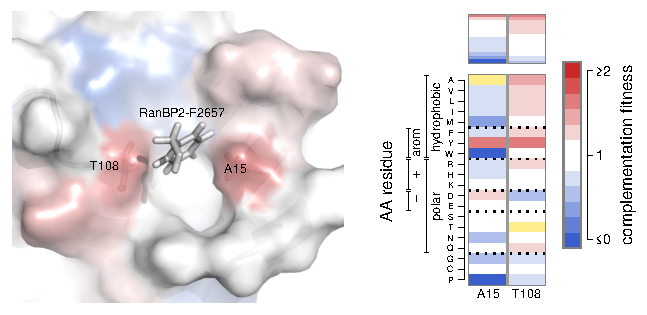
\includegraphics[width=\textwidth]{img/pi-stack.pdf}
	\caption{Potential de-novo pi-stack interaction between UBE2I and the E3 RanBP2. Structure data from \texttt{PDB:3UIP}~\cite{gareau_determinants_2012}}
	\label{fig:pi-stack}
\end{figure}

It is unclear how to interpret the effect of mutations that enhance growth in the yeast complementation assay. If fitness measured in the assay is directly proportional to fitness in the real biological context, then these enhancing mutations would be beneficial. However one can also imagine an alternative scenario in which activity-enhancing mutations are deleterious in the real biological context. To objectively distinguish between these possibilities, we collaborated with Jesse Bloom to employ a method he recently published that leverages likelihood-based phylogenetics to quantitatively compare how well different experimental measurements represent actual evolutionary constraints in nature~\cite{bloom_experimentally_2014,bloom_identification_2017}. We compared three models relating the experimental fitness to the evolutionary preference for a mutated amino-acid sequence: (a) the evolutionary preference was directly proportional to the untransformed experimental fitness; (b) the preference had a ceiling at the wildtype experimental fitness (values greater than 1 were set to 1); or (c) the preference was set to the reciprocal of fitness for mutations with greater-than-wildtype scores, corresponding to a deleterious effect of enhancing mutations. Dr. Bloom kindly provided the phydms software~\cite{bloom_identification_2017} to test which of these three approaches best described the evolutionary constraint on a set of naturally occurring \gene{UBE2I} homologs, using fitness scores that excluded conservation features from the regularization process, to avoid the circularity of using natural sequence data when deriving the scores. As shown in Table~\ref{tab:phydms}, the best fit is achieved using the model that assumes that enhancing mutations are deleterious. This result provides objective support for the idea that mutations that enhance activity above wildtype levels in the complementation assay are actually deleterious in a real biological context.

Based on these observations I reinterpreted cases of hyperactive complementation in the map as deleterious. I repeated the imputation and regularization procedure on the transformed map, which resulted in substantially improved cross-validation performance (Root-Mean-Squared-Deviation, RMSD, decreased from $0.33$ to $0.24$).

\begin{table}[h!]
	\centering
	\caption{Comparison of different models for the effects of hyperactivating mutations. AIC: Akaike Information Criterion\newline}
	\begin{tabular}{l r}
Model & \parbox[t]{1in}{$\Delta$AIC relative\newline to best model}\\ \hline\hline
Hyperactive mutations as deleterious & 0\\
Hyperactive mutations as WT & 27.7\\
Hyperactive mutations as beneficial	& 60.6	
	\end{tabular}
	\label{tab:phydms}
\end{table}



\subsubsection{Intragenic epistasis and compensatory mutations}

Full-length \gene{UBE2I} clones generated for DMS-BarSeq analysis often encoded more than one amino acid change. Multi-mutant clones offer the opportunity to search for intragenic genetic interactions. Genetic interaction is defined as the case of a combination of mutations that yields an unexpected phenotypic effect. Therefore, identifying genetic interactions requires modeling the phenotype that is expected from a combination of mutations, given the single-mutant effects.  Here I used a previously-described multiplicative model~\cite{phillips_language_1998,onge_systematic_2007} in which genetic interaction is measured as $\varepsilon_{ij} = f_i \cdot f_j - f_{ij}$, where $f_i$ and $f_j$ represent single mutant fitness and $f_{ij}$ represents double mutant fitness scores. Most double mutants (71\%) did not show a significant deviation from $\varepsilon_{ij} = 0$ under this model, while 328 position pairs did show significant genetic interaction (Figure~\ref{fig:epsistasis}).

Of particular interest are compensatory interactions, i.e. cases where a double mutation is more fit than either of the component single mutations.  Where compensatory residues are proximal in the protein structure, the combination of two mutant residues may be able to re-establish a physical interaction that was lost in each of the single mutants. Although the majority of genetically interacting sites were not proximal in the structure (Figure~\ref{fig:epsistasis}B), there were interesting exceptions. For example, the I4T-P69S double mutant appears to exhibit compensatory behaviour: In the wild type structure, the van-der-Waals radii of the two residues are in direct contact (Figure~\ref{fig:epsistasis}C). Either mutation alone would be expected to destabilize the hydrophobic interaction between isoleucine and proline.  However, in the double mutant, hydroxyl groups on the two residues could adopt a hydrogen bond that re-establishes interaction and re-stabilizes the fold (Figure~\ref{fig:epsistasis}D).

\begin{figure}[h!]
	\centering
	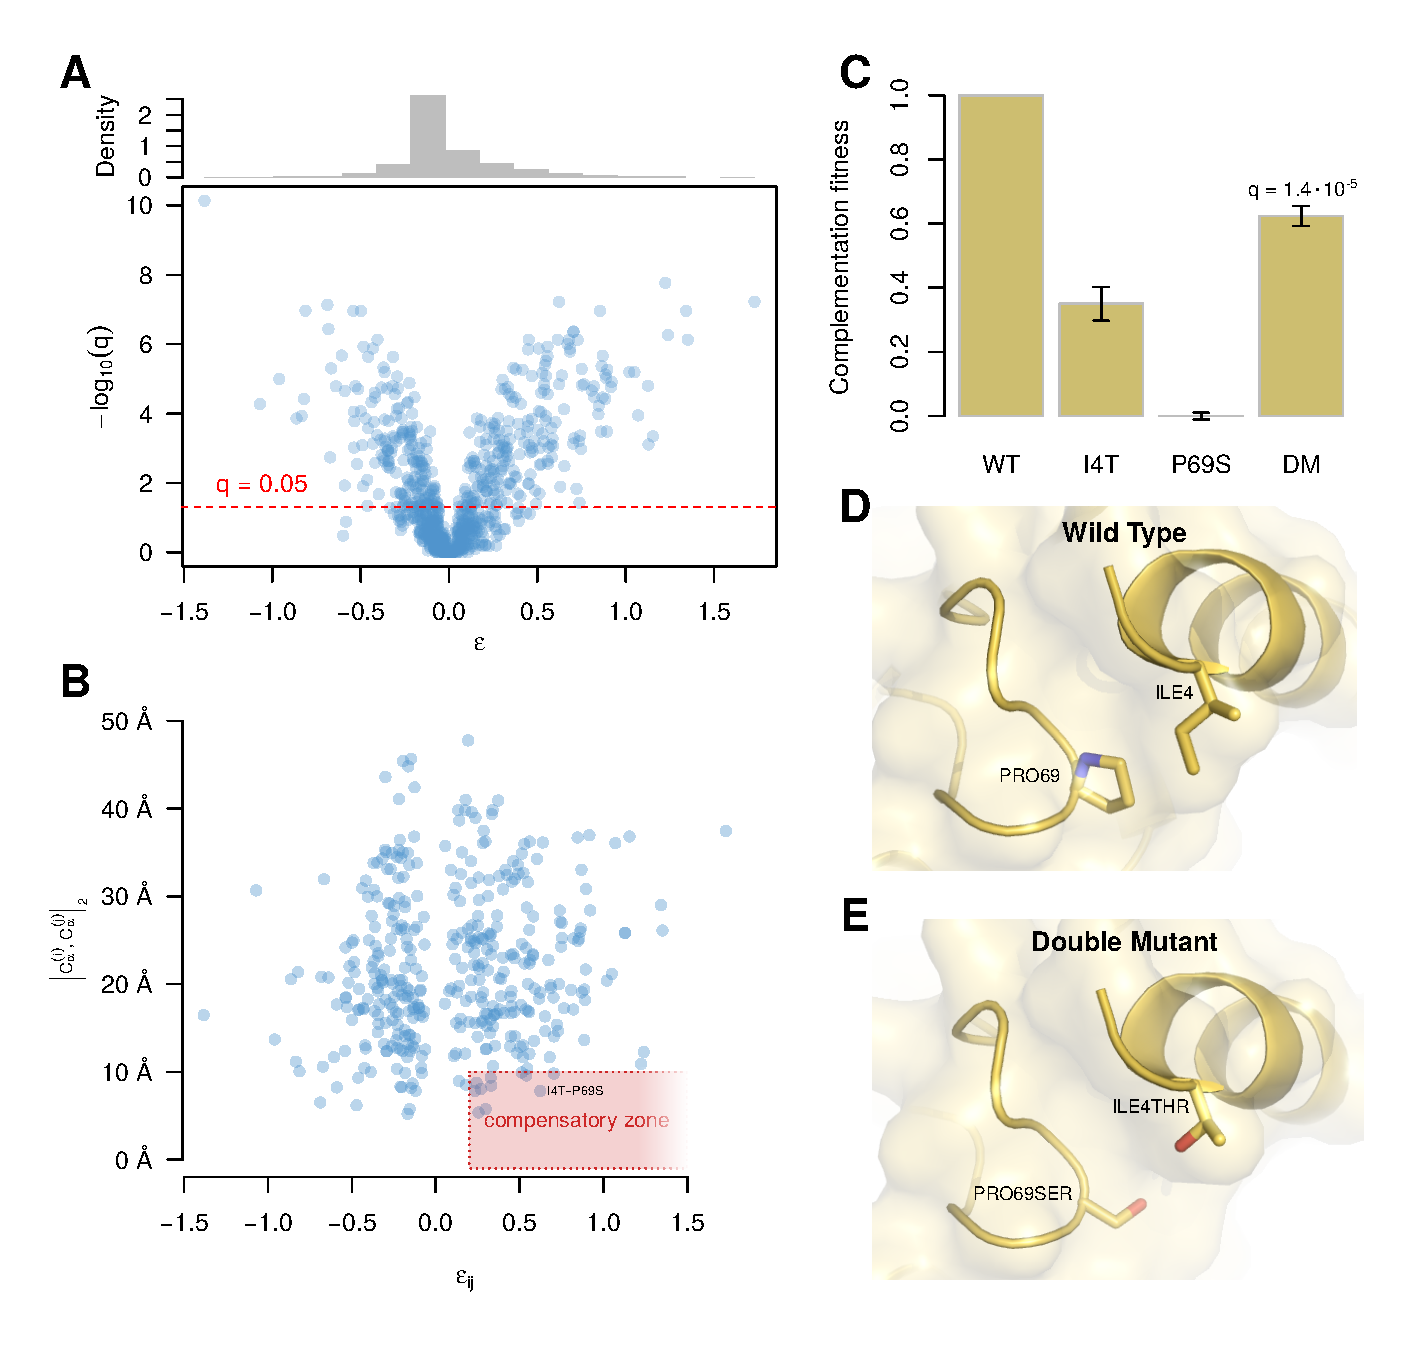
\includegraphics[width=\textwidth]{img/epistasis.pdf}
	\caption{Intragenic epistasis in UBE2I. A) Volcano plot of epsilon values (deviation from expectation) vs FDR-corrected significance levels. Above: Histogram of epsilon values. B) Comparison of epsilon values with inter-alpha-carbon distance in the 3D structure. C) Positive genetic interaction between I4T and P69S. The double mutant fitness (DM) significantly exceeds that of both single mutants and their product. D) Wiltype structural context for I4 and P69. E) Simulated double mutant structural context.}
	\label{fig:epsistasis}
\end{figure}


\subsection{A comparison of complementation and Y2H reveals a interaction interface}

An important factor behind the choice of UBE2I as a testing ground for the DMS framework was the mechanistic complexity of the Sumoylation pathway, in which the central component UBE2I engages in many different protein-protein interactions. Having examined the relative importance of its known interaction interfaces we wished to evaluate the possibility of detecting new interfaces. To this end, we adapted the DMS framework to use a Y2H assay in the selection step.

% mut	 compl	 ia
% C75F	 1.6644	-0.162
% C75S	 0.9952	 0.493
% F155L	 0.7357	 0.154
% F155V	 0.9469	 0.031
% I45T	 0.7809	 0.254
% L113I	 0.9961	 0.460
% L114F	 0.9427	 0.437
% L81V	 0.9363	 0.374
% P128S	 1.1586	 0.377
% P157A	 1.1586	 0.296
% P73T	 0.7786	 0.143
% Q126E	 1.1710	 0.277
% R61P	 0.6716	-0.347
% V25L	 0.6808	 0.123
% V25M	 0.7794	 0.090

We explored the set of previously identified Y2H interactions of UBE2I and found its interaction with the Special AT-rich sequence Binding protein SATB1, a sumoylation target~\cite{tan_sumo_2008}, to be the strongest interaction signal. We used DMS-BarSeq to map the effects of UBE2I variants on the UBE2I-SATB1 interaction and compared the results to those of the complementation assay. Although too few variants in the Y2H screen were measured with high enough confidence to perform reliable imputation, I was able to identify 15 variants that specifically disrupted the UBE2I-SATB1 binding without affecting its overall function as measured by the complementation assay. Interestingly, three amino acid positions (V25, C75 and F155) were represented with multiple variants in this list, highlighting their importance. Figure~\ref{fig:y2hVScompl} marks the affected residues on the surface of UBE2I, which may determine the specificity of the UBE2I-SATB1 interaction. Consistent with SATB1's known role as a sumoylation target~\cite{tan_sumo_2008}, the residues are clustered near the known substrate recognition and binding surface. Intriguingly, I also found a number of residues within UBE2I's hydrophobic core, that upon mutation to alternative hydrophobic residues resulted in a disruption of UBE2I-SATB1 binding (Figure~\ref{fig:y2hVScompl}). The fact that these residues are physically close to the locations of surface residues with similar behaviour may indicate that mutations at these positions could result in subtle shifts of UBE2I's fold that disrupt the SATB1 binding interface without affecting other functions.

\begin{figure}[h!]
	\centering
	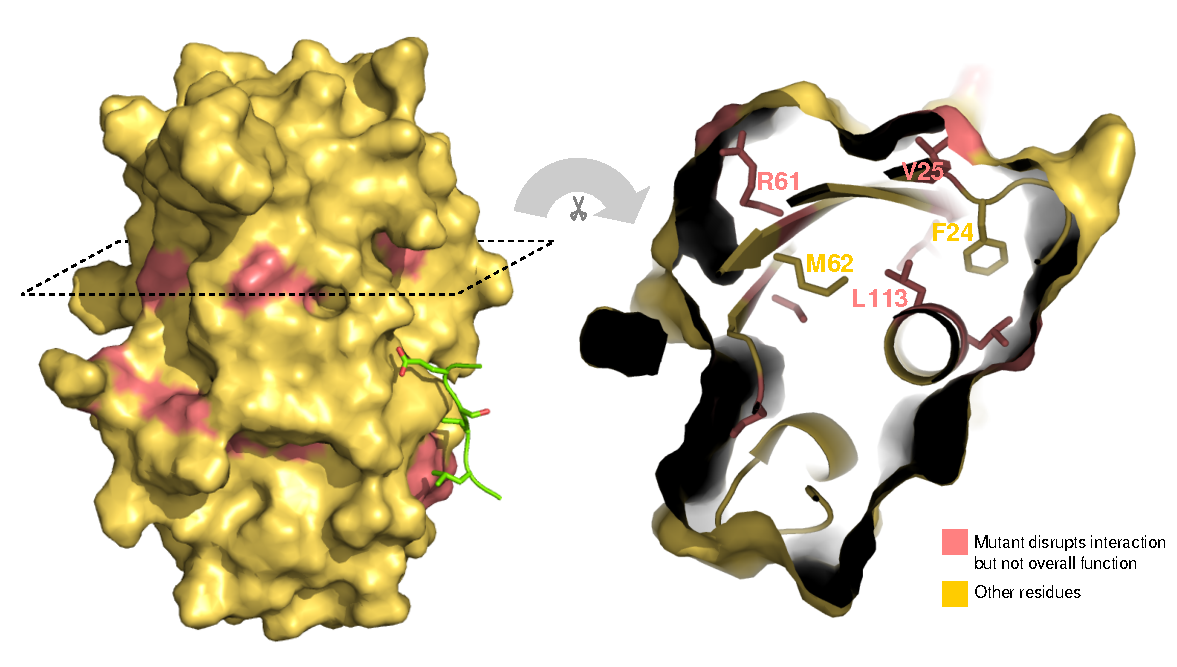
\includegraphics[width=\textwidth]{img/satb1_interface.pdf}
	\caption{Potential interfacial residues for UBE2I's interaction with SATB1. Highlighted residues disrupt Y2H interaction without disrupting overall function as measured by complementation. The dotted frame in the left panel indicates the plane across which the structure was cut to produce the panel on the right.}
	\label{fig:y2hVScompl}
\end{figure}


\subsection{A functional map for SUMO1}

Using the DMS-TileSeq version of the framework established in the previous chapter we also created a complete functional map for SUMO1 (Figure~\ref{fig:sumo-map}A). Out of the 1919 possible amino acid changes, fitness effects for 1700 (89\%) were measured directly in the complementation competition experiment. The remaining 11\% were obtained through imputation, which achieved a cross-validation RMSD of 0.25, a performance very similar to that of the UBE2I map.

The most immediately apparent feature of the SUMO1 map was the strong enrichment for neutral substitutions within the first 20 amino acid positions, which is consistent both with the low level of evolutionary conservation for this region and its annotation as a disordered region. The last four amino acid positions appeared similarly insensitive to mutation, consistent with the cleavage of this region by SENP proteases during SUMO maturation. By contrast, other residue positions were strongly sensitive to mutation, including many inward-facing residues that are apparently constrained to be hydrophobic. As expected, the C-terminal diglycine, directly preceding the last four cleaved residues, is also very sensitive to mutation, as it is required for the covalent binding of SUMO to the E1, the E2 and to the sumoylation target protein. Interestingly, except for the C-terminal diglycine, the residues that directly touch the E2 during covalent binding are not as sensitive (Figure~\ref{fig:sumo-map}B). This may be due to  SUMO being force-fed to the E2 by the E1 activating complex and the thioester bond it forms with the E2's cysteine 93 being sufficient to maintain the complex. By contrast, residues in the interface for non-covalent E2 binding are much more sensitive (Figure~\ref{fig:sumo-map}C), especially leucine 80 and methionine 82.

Other strongly constrained residues are core members of interaction interfaces. These include the central phenylalanine 36 in the SUMO recognition motif (SRM) interface; glycine 68, which forms the apex of a tight turn within the interface with de-sumoylation enzymes, as well as the E1 and E2 proteins; and leucine 80, which is part of the interface with non-covalently bound E2. 

\begin{figure}[h!]
	\centering
	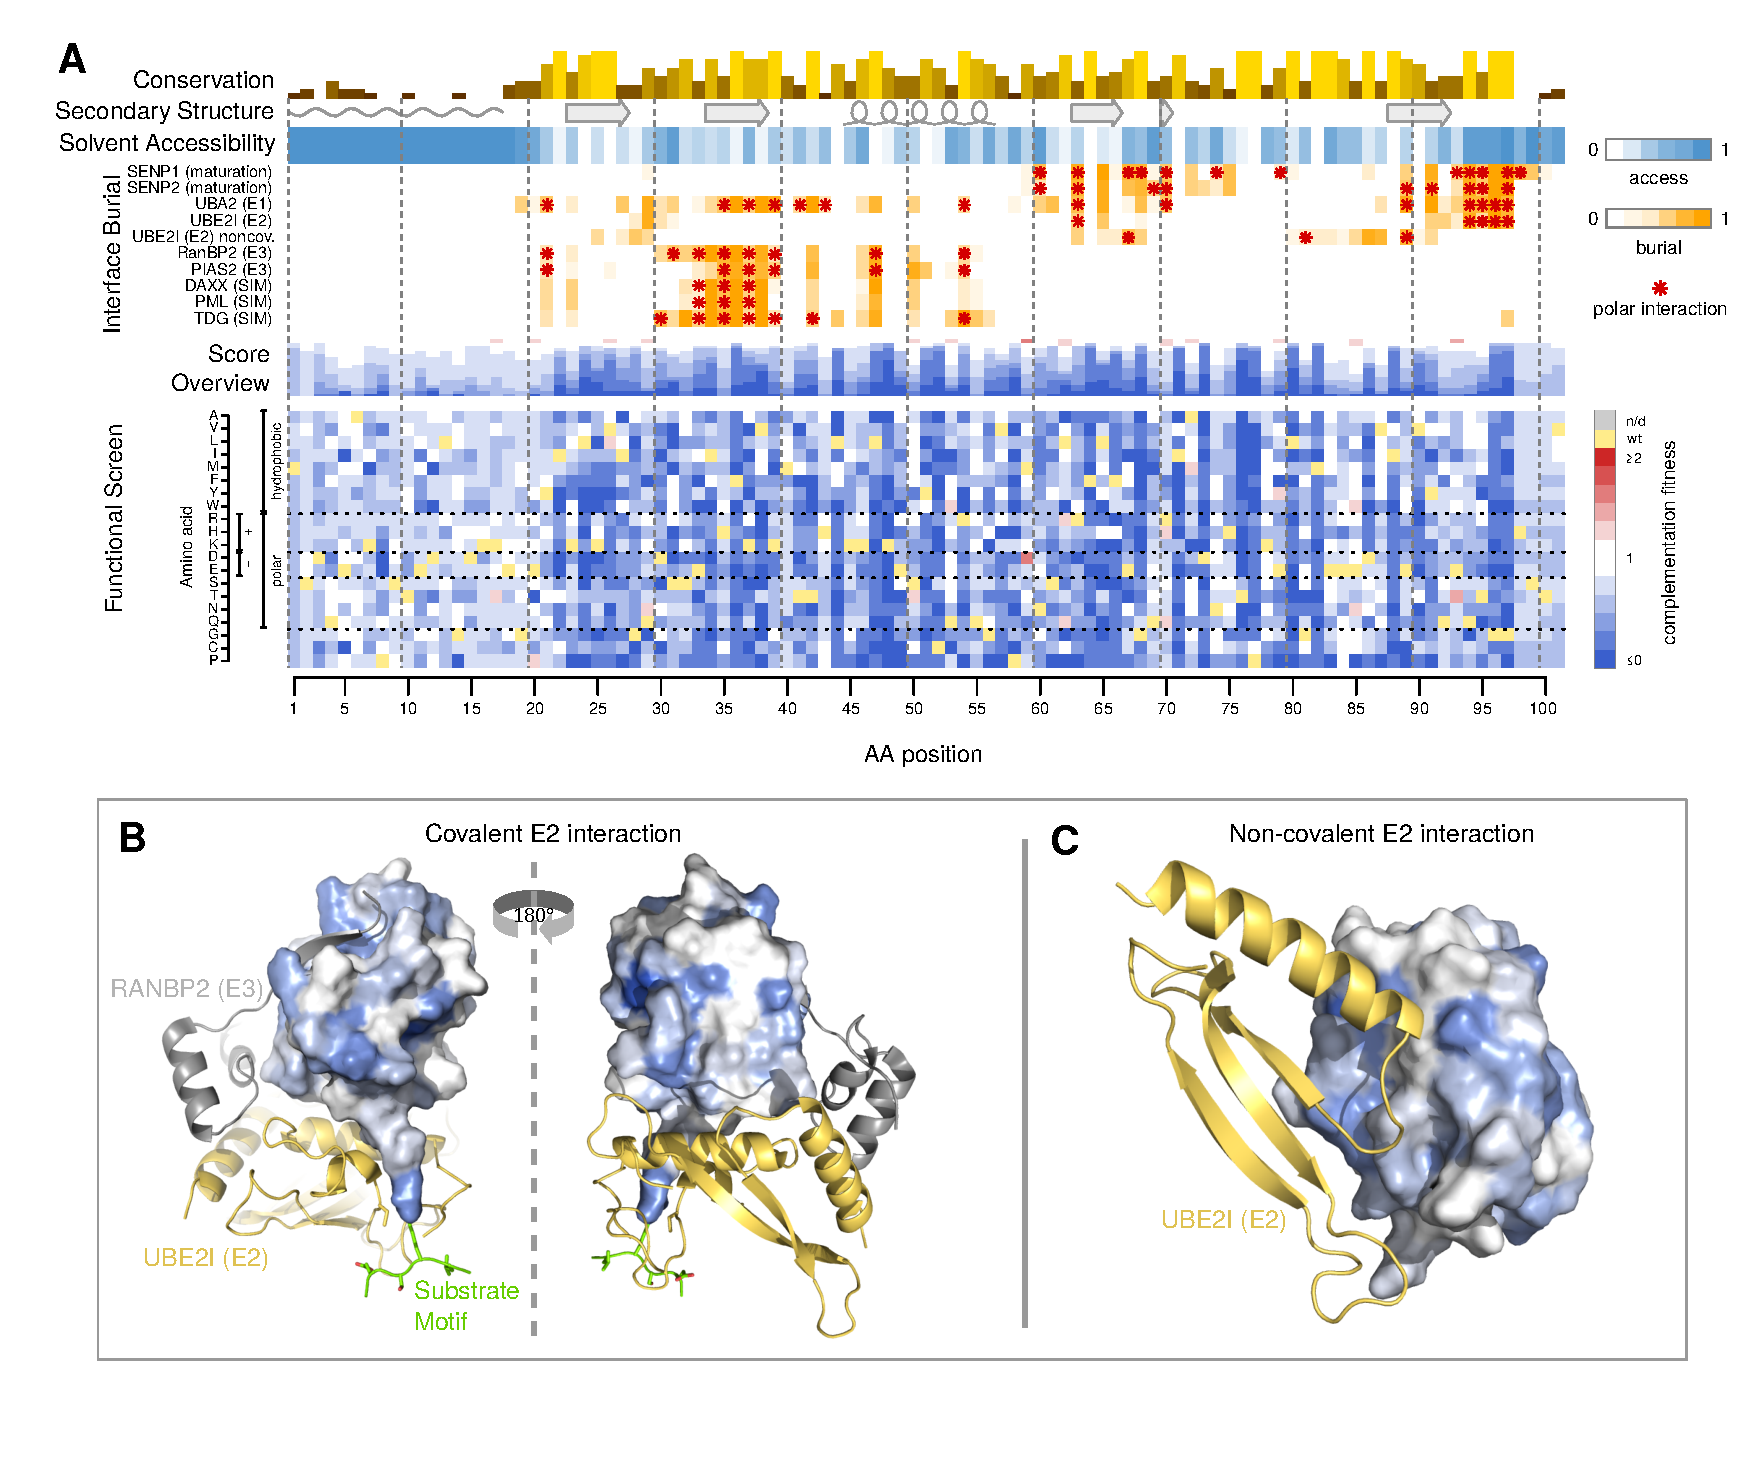
\includegraphics[width=\textwidth]{img/sumo-map.pdf}
	\caption{Functional map of SUMO1. A) From top to bottom: Position-wise evolutionary conservation; Secondary structure; Relative solvent accessibility; Relative burial in interaction interfaces with SENP1, SNEP2, UBA2, UBE2I (covalent binding), UBE2I (noncovalent binding), RanBP2, PIAS2, DAXX, PML, and TDG; breakdown of relative amounts of variants with different complementation scores; Heatmap of individual amino acid change effects on complementation fitness. B) SUMO1 structure coloured according to median complementation fitness score. Partial structure of covalently bound UBE2I shown in golden cartoon representation, $\Psi$KxE substrate recognition motif shown in green stick representation C) Colors as in B, but partial structure of UBE2I is shown in non-covalent binding mode.}
	\label{fig:sumo-map}
\end{figure}

The proximity and orientation of aspartate 73 and lysine 48 suggests that they are able to form a salt bridge with one another.  The importance of each residue according to the DMS map supports a model in which this salt bridge is important for SUMO folding and/or stability. Interestingly, substituting aspartate for methionine 59, which points towards lysine 48 from an angle similar to that of aspartate 73, enhances the complementation fitness of SUMO1 beyond wild type levels.  This further underlines the potential importance of a polar interaction involving lysine 48 (Figure~\ref{fig:saltbridge}).

\begin{figure}[h!]
	\centering
	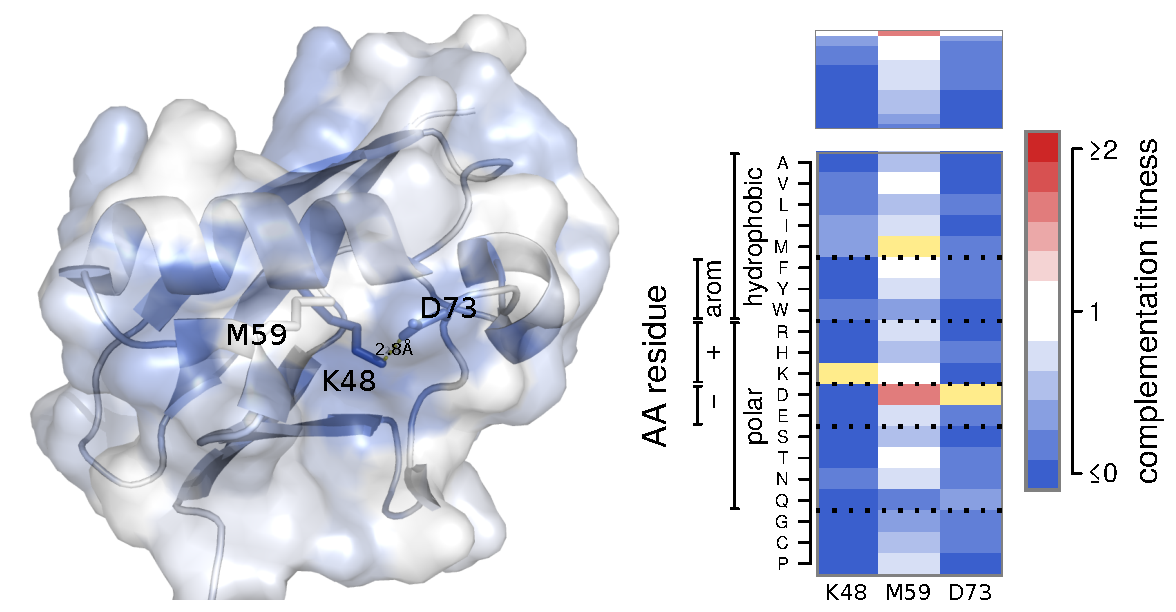
\includegraphics[width=\textwidth]{img/saltbridge.pdf}
	\caption{A salt bridge within SUMO1 between Asp73 and Lys38 appears important for stability. Met59Asp may increase stability even further.}
	\label{fig:saltbridge}
\end{figure}


% As was shown above for UBE2I, phylogenetic analysis of SUMO1 similarly showed that adaptive mutations with ability to complement yeast better than wild-type are likely deleterious in humans. We therefore transformed fitness scores so that such adaptive mutations are considered to be deleterious (see Methods).  However, because adaptive substitutions may provide interesting clues about differences between yeast and human cellular contexts, we provide both transformed (Figure 5) and untransformed versions of each map.




\subsection{Functional maps of three human disease genes}

Having established and evaluated the Deep Mutational Scanning framework on two members of the sumoylation pathway, we aimed to create maps for a diverse set of genes that have been associated with disease with varying degrees of confidence. While  heterozygous null mutations in SUMO1 have previously been associated with cleft palate~\cite{andreou_tbx22_2007}, we wished to create maps that could be tested in the context of variant classification in terms of disease. Based on the availability of robust complementation assays, we applied DMS-TileSeq to the following protein targets: Thiamine Pyrophosphokinase 1 (TPK1), associated with vitamin B1 metabolism dysfunction~\cite{mayr_thiamine_2011}; Neuronal Calcium Sensor 1 (NCS1), which has been implicated in autism based on a single \textit{de novo} mutation~\cite{handley_structural_2010};  and CALM1, CALM2 and CALM3 associated with the heart conditions long-QT syndrome~\cite{crotti_calmodulin_2013} and catecholaminergic polymorphic ventricular tachycardia~\cite{nyegaard_mutations_2012}. Although the three calmodulin genes differ in nucleotide sequence, each encodes the same polypeptide sequence. Thus, we performed a deep mutational scan only for CALM1, which enabled us to also map missense variant effects in CALM2 and CALM3. In each case, we used the TileSeq approach coupled with complementation to generate a map of missense variant functions. 


\begin{table}
	\centering
	\caption{Map quality comparison. RMSD: Root-Mean-Squared-Deviation in $10\times$ cross validation. $\max(\sigma_{\bar{x}})$: maximal standard error across non-imputed values in the map.\newline}
	\begin{tabular}{l p{.9in} p{.9in} p{1in} p{1in} p{1in}}
\textbf{Gene} & 
\textbf{Possible AA~changes} & 
\textbf{Achieved AA~changes} & 
\textbf{Imputation RMSD} & 
\textbf{Experimental $\max(\sigma_{\bar{x}})$} & 
\textbf{Regularized $\max(\sigma_{\bar{x}})$} \\ \hline\hline
\textbf{UBE2I} & 3021 & 2563 (85\%) & 0.24 & 0.36 & 0.25 \\
\textbf{SUMO1} & 1919 & 1700 (89\%) & 0.25 & 0.19 & 0.17 \\
\textbf{TPK1} & 4617 & 3181 (69\%) & 0.34 & 0.49 & 0.37 \\
\textbf{CALM1} & 2831 & 1813 (64\%) & 0.29 & 0.28 & 0.22 \\
\textbf{NCS1} & 3610 & 2542 (70\%) &  0.63 & 1.84 & 0.97
	\end{tabular}
	\label{tab:summary}
\end{table}



As was shown above for UBE2I, phylogenetic analysis of SUMO1 similarly showed that variants with ability to complement yeast better than wild-type are likely deleterious in humans. I therefore transformed fitness scores so that such hypercomplementing mutations are considered to be deleterious (see Methods). The transformed disease gene maps can be seen in Figures \ref{fig:tpk1-map} and \ref{fig:calm+ncs1-maps}.  However, since hypercomplementing substitutions may provide interesting clues about differences between yeast and human cellular contexts, I also provide untransformed versions of each map (see Appendix~\ref{apdx:maps}).

%%FIGURE: Map for TPK1/NCS1/CALM1


\subsubsection{A thiamine pyrophosphokinase map reflects a recessive phenotype}

Thiamine pyrophosphokinase (TPK1) is a protein that forms a dimer to perform its biochemical function. Its substrate, thiamine diphosphate, is bound within two active sites formed by the dimerization interface~\cite{timm_crystal_2001}. That is, each monomer contributes half of the residues making up each of the two active sites.  Each monomer in turn is made up of an N-terminal globular domain and a C-terminal $\beta$-sandwich domain (Figure~\ref{fig:tpk1_structure}A). The residues most sensitive to mutation in the protein make up the hydrophobic cores of the two domains: L21, V22, W36, G48, Y53, P65, G70, Y83, L108, I122, T124, and G127 for the N-terminal domain; and L161, G168, G199, L200, V227, V229, L236, and W237 for the C-terminal domain (Figure~\ref{fig:tpk1_structure}B). 

\begin{landscape}
\begin{figure}[h!]
	\centering
	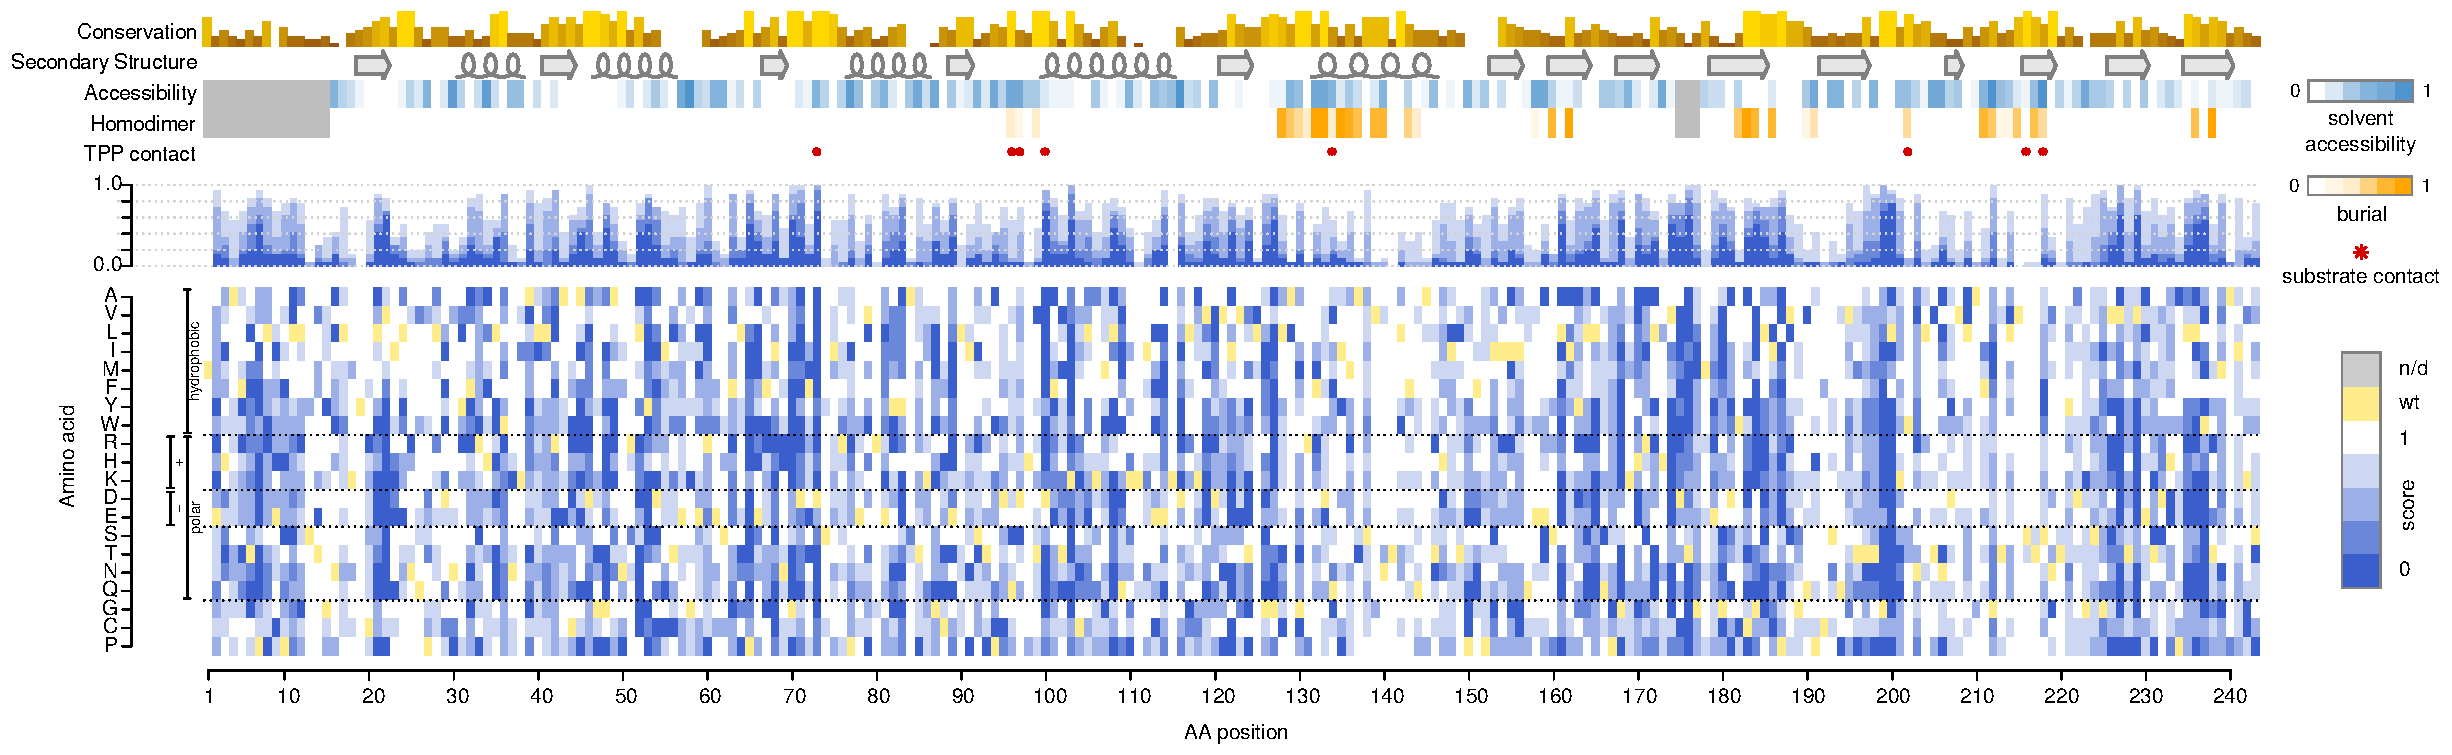
\includegraphics[width=9in]{img/tpk1-map.pdf}
	\caption{Functional map of Thiamine pyrophosphokinase 1 (TPK1). From top to bottom: Position-wise evolutionary conservation (AMAS); Secondary structure; Relative solvent accessibililty; Relative burial in homodimerization interface; Contacts with Thiamine diphosphate; Summary track showing the shares of amino acid changes resulting in varying degrees of fitness effects; Detailed heatmap showing individual amino acid change effects.}
	\label{fig:tpk1-map}
\end{figure}
\end{landscape}

\begin{figure}[h!]
	\centering
	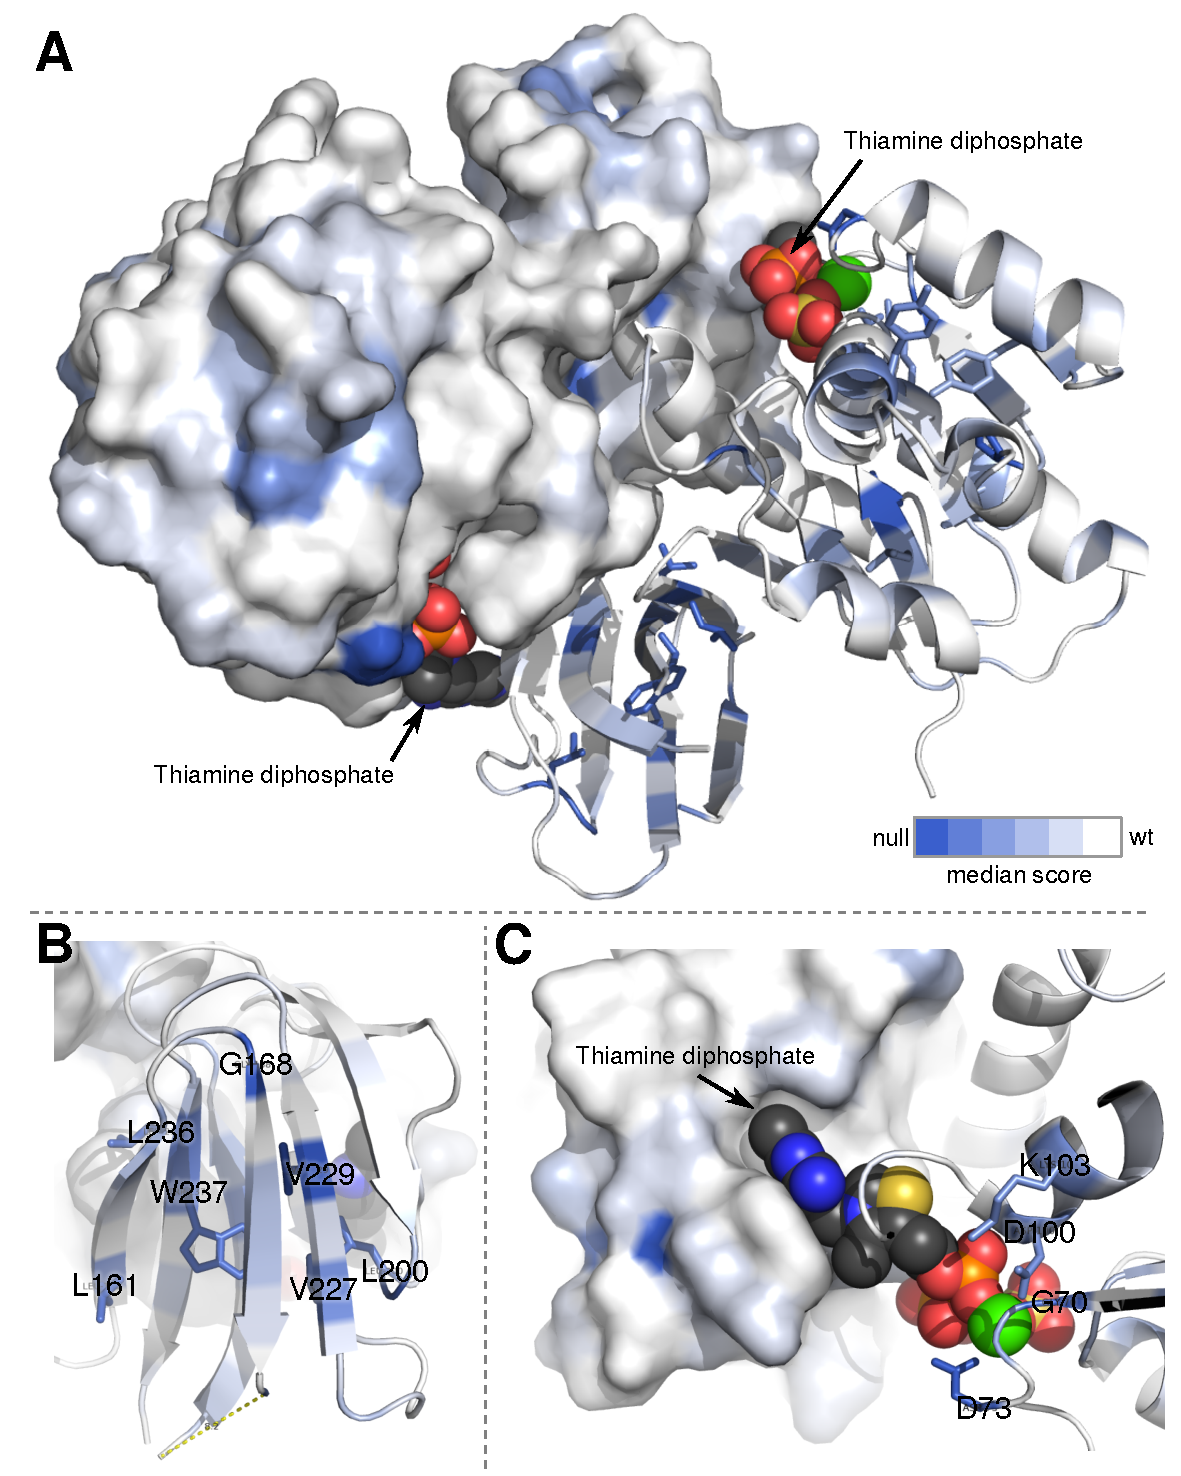
\includegraphics[width=.8\textwidth]{img/tpk1_structure.pdf}
	\caption{Thiamine pyrophosphokinase 1 coloured by median complementation score. A) TPK1 homodimer structure showing one monomer as surface model, the other monomer as cartoon model. B) Hydrophobic residues facing the inside of the C-terminal $\beta$-sandwich domain are sensitive to mutation. C) Active site residues in contact with the substrate are sensitive to mutation. Structure data from \texttt{PDB:3S4Y}~\cite{timm_crystal_2001}}
	\label{fig:tpk1_structure}
\end{figure}

As might have been expected, mutation-sensitive residues include those closely involved in forming the active sites: D46, G70, D71, D73, D100, and K103 in the N-terminal half of the active site, contacting the diphosphate portion of the substrate (Figure~\ref{fig:tpk1_structure}C). In the C-terminal half of the active site, K203, L209, G212, L214, S216, T217, and N219 show similar sensitivity. Interestingly, the tryptophan residue at position 202 appears to be insensitive to mutation despite its close and extensive contact with the thiamine ligand. By contrast, a neighbouring lysine at position 201 is surprisingly sensitive suggesting potential importance in coordinating the ligand.  The remainder of the dimerization interface also features a number of sensitive residues, such as M136, G184, V188, G189 and G211. Finally, residues 1-12, which form a $\beta$-strand anchoring the N-terminal domain back to the C-terminal domain were also found to be sensitive.

\subsubsection{The two calcium sensors NCS1 and Calmodulin show different profiles}

Calmodulin (CALM1/2/3) and the Neuronal Calcium Sensor protein (NCS1) are homologs (E-value $4 \cdot 10^{-5}$ when searched against the human proteome~\cite{altschul_basic_1990,the_uniprot_consortium_uniprot:_2015}) with 24\% sequence identity and 48.5\% similarity~\cite{rice_emboss:_2000}. However, they display different impact patterns despite their similar domain structure and similar molecular roles as calcium sensing proteins. Both are comprised of four Calcium-binding EF-hands, with NCS1 containing additional sequences upstream and downstream of the four hands. A comparison of previously published NMR structures reveals that the overall folds of the two proteins differ substantially~\cite{sarhan_crystallographic_2012,heidarsson_c-terminal_2012}. Calmodulin features a long central helix that separates two globular domains, called the N-lobe and the C-lobe, each comprised of two EF hands. A hydrophobic pocket serving as a binding interface for interacting proteins is nested within the C-terminal domain. NCS1, by contrast, forms a single shell-like shape, centered around a large hydrophobic crevice. This crevice acts as a binding interface for interacting proteins. Thus, the divergent DMS profiles observed for CALM1/2/3 and NCS1 are consistent with these substantial structural differences.

The Neuronal Calcium Sensor NCS1 displays the greatest sensitivity to mutation within the N-terminal region containing the myristoylation site.  This myristoylation site is essential for anchoring NCS1 into the plasma membrane. One other residue that stands out is the tryptophan at position 30, which results in complete loss of function when replaced with any other amino acid. Like most other sensitive residues W30 is found among those contributing to the hydrophobic crevice acting as an interaction interface. Other cases include F55, F56, A104, M121, I152, and A182. An interesting observation can be made with respect to the two helices that separate the two N-terminal EF hands from the two C-terminal EF hands. A kink between the two helices brings them into an angle that allows the globular shape of the overall protein to form. Without this kink it is conceivable that NCS1's fold would much more resemble that of Calmodulin. A glycine residue (G95) is likely responsible for forming that kink due to its helix breaking properties. This residue is also found to be quite sensitive to mutation.

\begin{landscape}
\begin{figure}[h!]
	\centering
	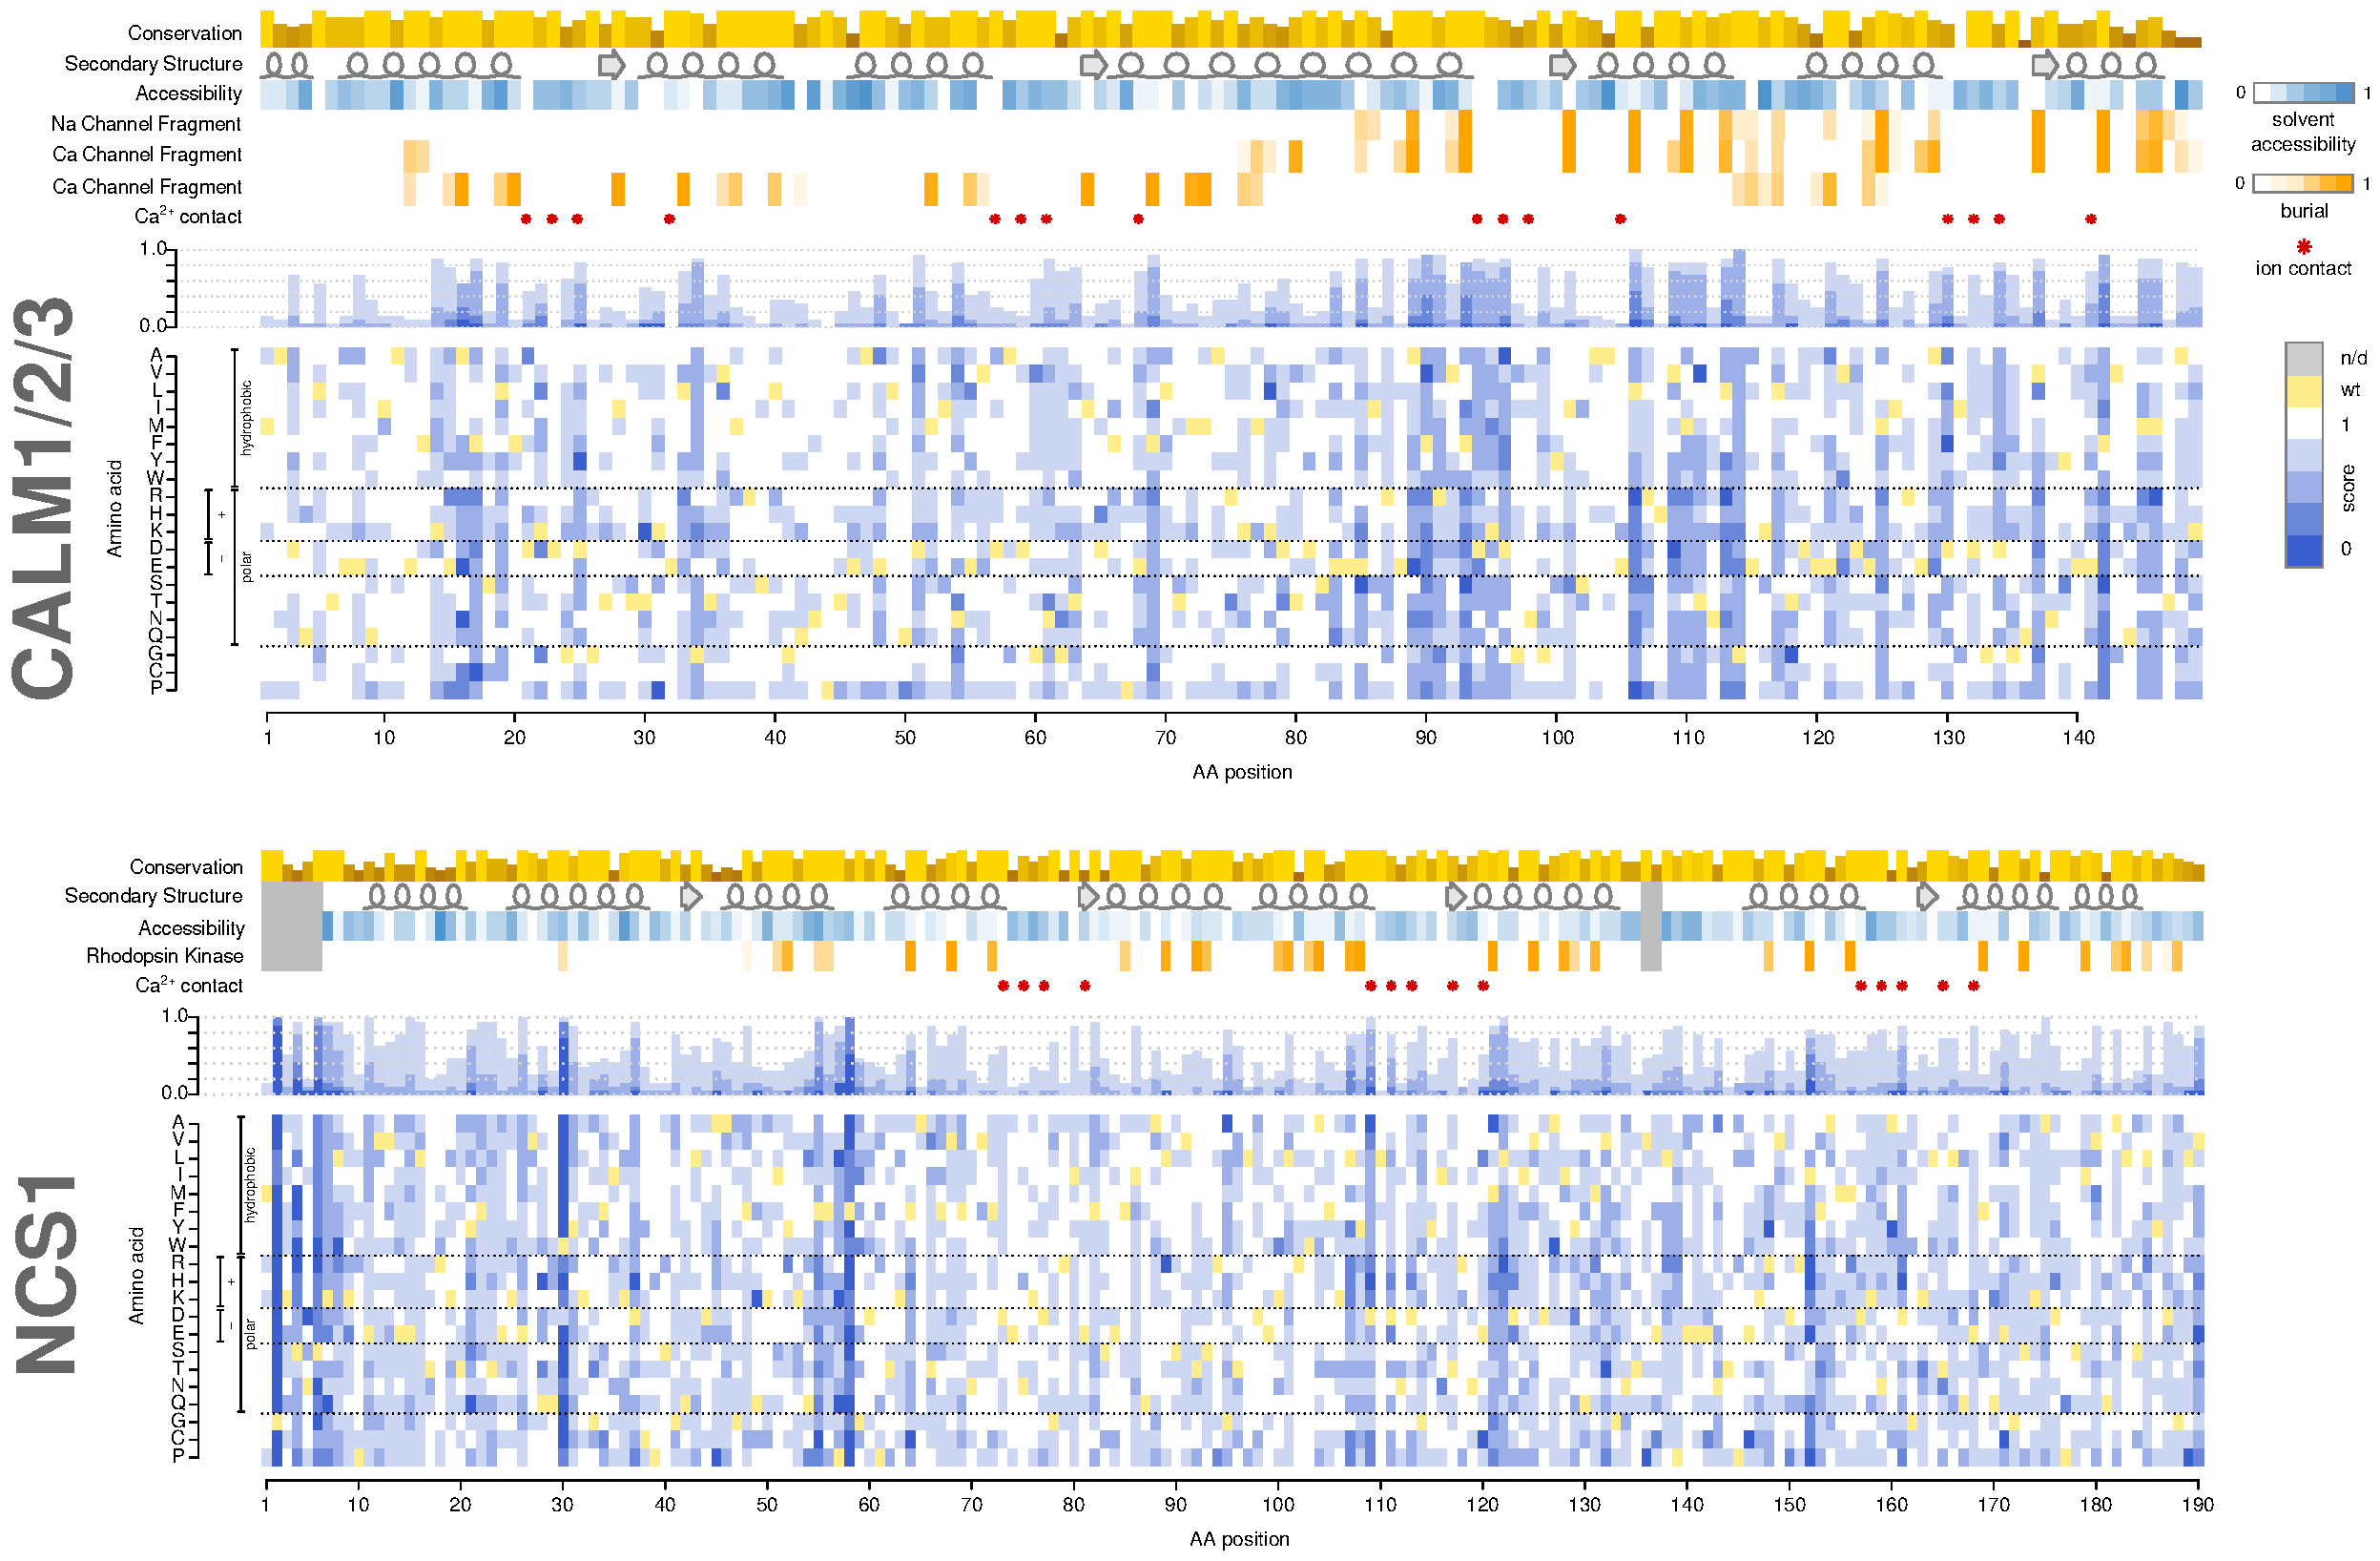
\includegraphics[width=9in]{img/calm+ncs1-maps.pdf}
	\caption{Functional map of Thiamine pyrophosphokinase 1 (TPK1). From top to bottom: Position-wise evolutionary conservation (AMAS); Secondary structure; Relative solvent accessibililty; Relative burial in homodimerization interface; Contacts with Thiamine diphosphate; Summary track showing the shares of amino acid changes resulting in varying degrees of fitness effects; Detailed heatmap showing individual amino acid change effects.}
	\label{fig:calm+ncs1-maps}
\end{figure}
\end{landscape}

Within Calmodulin, the regions most sensitive to mutation are: 1) the hydrophobic cores of the two globular domains; 2) interfacial residues for protein-protein interactions, and 3) a subset of the negatively charged residues in EF hands that contact Ca$^{2+}$ ions. Within the hydrophobic cores of the two lobes, five mutually interacting phenylalanine residues at positions 17, 69, 90, 93, and 142 stand out in particular, as all of them are found in the top 9 most sensitive residues on the map. Within the interaction interface, the residues D85, A89, F93, M100, L106, V109, L113, G114, L117, M125, V137, F142, M145, M146 are the most strongly sensitive to mutation. Regarding the four Calcium-binding EF-hand loops, it was interesting to find that only a subset of the negatively-charged residues contacting Ca$^{2+}$ are even moderately sensitive. Within EF1, only D25 appears to be important, in EF2 only N61, in EF3 only D94 and D96, and in EF4 only D130 and D134. Overall, the EF3/4 in the C-lobe also appear to be more important than their N-lobe counterparts. This is in agreement with previous observations made by Sarhan and colleagues~\cite{sarhan_crystallographic_2012}, who described the C-lobe as the primary sensory mechanism. A number of unexplained sensitivities exist as well: Arginines at positions 54 and 91 show strong phenotypes despite extending from seemingly unused surfaces of the protein, offering the possibility that these residues are functionally relevant sites of interaction or modification.



\subsection{Functional maps recapitulate known disease cases}

To validate the utility of the maps in the context of human disease, I extracted known disease-associated variants from ClinVar~\cite{landrum_clinvar:_2016}, as well as rare and common polymorphisms observed independent of disease from GnomAD~\cite{lek_analysis_2016}, and somatic variants previously observed in tumors from COSMIC~\cite{forbes_cosmic:_2001}. 

For TPK1, a large number of very rare variants (minor allele frequency or $\text{MAF} < 10^{-6}$) is known from GnomAD. At first look, it appears the majority of these variants are shown to be deleterious (Figure~\ref{fig:tpk1_diploid}). This seems unlikely, given that Thiamine Metabolism Dysfunction Syndrome, reported to be caused by mutations in this gene, is a very severe disease to which patients succumb in childhood~\cite{mayr_thiamine_2011}., and that GnomAD attempts to filter out subjects with severe pediatric disease. However, the disease is also known to follow a recessive inheritance pattern, with only homozygous or compound heterozygous individuals being affected. I thus used phased sequence data from the 1000 Genomes Project~\cite{the_1000_genomes_project_consortium_global_2015} to determine the diploid genotypes in the TPK1 locus for all listed individuals and based the phenotype predictions on the maximum fitness score of either allele. This improved prediction performance markedly, leading to complete separation between disease and non-disease genotypes. However, both PROVEAN and PolyPhen-2 were also able to perfectly separate the two groups (Figure~\ref{fig:tpk1_diploid}B), so that additional compound heterozygotes with known disease status will be required to determine whether this DMS map is more useful than computational methods for classifying pathogenic TPK1 variants. 

\begin{figure}[h!]
	\centering
	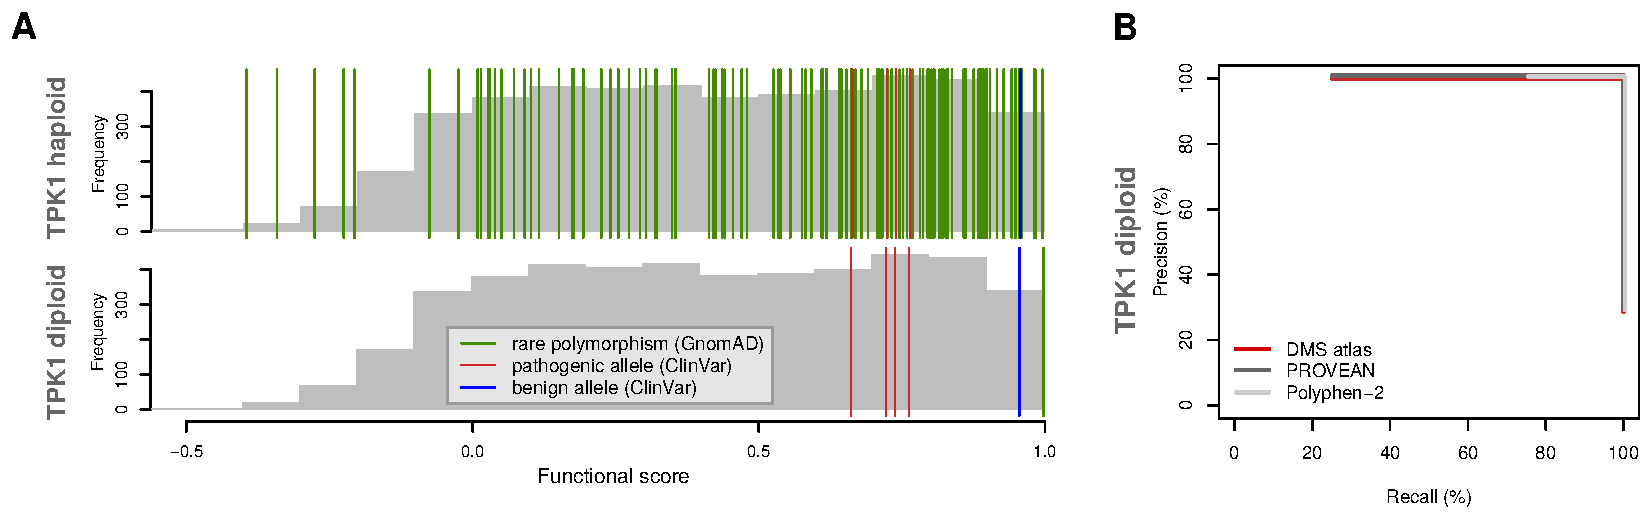
\includegraphics[width=\textwidth]{img/diploid.pdf}
	\caption{Variant classificationin TPK1. A) Distribution of functional scores for rare polymorphisms (GnomAD) (green) and pathogenic and benign variants (ClinVar) (red, blue) in TPK1 overlaid on a histogram of functional scores for all missense variant. Top panel: Haploid scores considering the phenotype based only on a single allele. Bottom panel: Diploid scores, considering the phenotype based on both alleles in each individual. B) Precision-Recall curve for disease variant classification using diploid scores from the atlas presented here, PROVEAN and PolyPhen-2, based on the data from (A).}
	\label{fig:tpk1_diploid}
\end{figure}


While NCS1 does not have any entries in ClinVar, a previous publication identified the variant R102Q as a \textit{de novo} variant in a single patient with autism spectrum disorder~\cite{handley_structural_2010}. While the variant did not affect overall protein folding and localization, the authors did observe that the dynamics of cytosol-membrane cycling were altered. The complementation map did not show any functional impact for this variant.

Similarly, no disease-associated missense alleles are known for UBE2I and SUMO1 in ClinVar. However, a number of somatic mutations for all three genes have been observed in cancer according to COSMIC. While these can be expected to passenger mutations, one may still hypothesize that somatic variants are likely not subject to the same selection pressures as germline variants, as interference with developmental processes is not necessarily detrimental to a tumour. I thus tested whether germline polymorphisms in these three genes were enriched for being functional compared to their somatic counterparts in the maps. Indeed, I observed a significant difference between the two sets (Wilcoxon $P = 2.6 \cdot 10^{-5}$) (Figure~\ref{fig:calm_disease}C).

Finally, I examined the functional map of Calmodulin and found that it was able to distinguish disease variants from non-disease variants very well (Figure~\ref{fig:calm_disease}A). In contrast to TPK1, the Calmodulin map did not need to be corrected for diploid genotypes, as previously reported disease variants have been described as following a dominant inheritance pattern~\cite{crotti_calmodulin_2013}. A precision-recall (PRC) plot reveals a superior performance (AUC = 0.74) compared to PROVEAN (AUC = 0.47) and PolyPhen-2 (AUC = 0.47).  

\begin{figure}[h!]
	\centering
	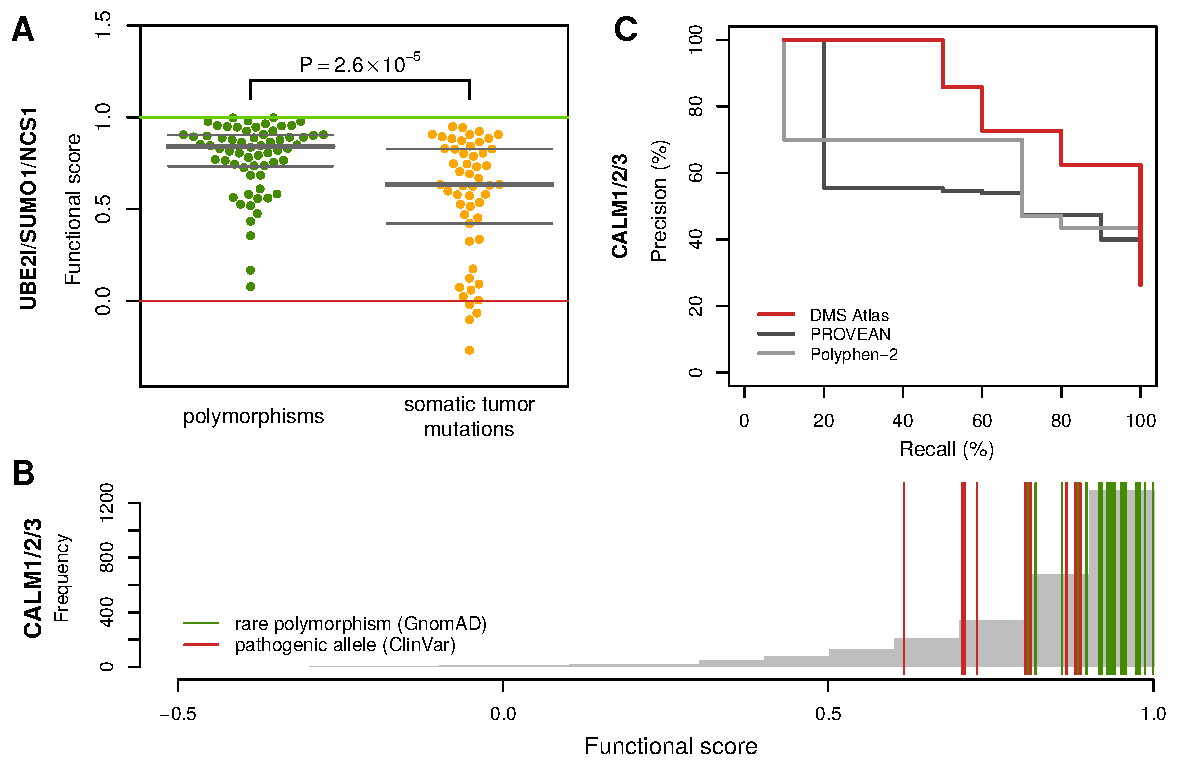
\includegraphics[width=\textwidth]{img/calm_disease.pdf}
	\caption{Detection of disease-associated variants. A) Distributions of functional scores for rare polymorphisms (GnomAD) (green) and for somatic in cancer (COSMIC) (gold) in UBE2I, SUMO1 and NCS1. B) Distribution of functional scores for rare polymorphisms (GnomAD) (green) and known pathogenic alleles (ClinVar) (red) in CALM1, CALM2 and CALM3, overlaid on a histogram of all missense variant scores (gray). C) Precision-Recall curves for classification of disease variants using the variant atlas presented here, PROVEAN and PolyPhen-2 in CALM1, CALM2 and CALM3 based on rare polymorphisms from GnomAD and pathogenic variants from ClinVar.}
	\label{fig:calm_disease}
\end{figure}


To further put the Calmodulin map to the test in a clinical scenario, we inquired with Invitae, a company offering gene panel sequencing services for Long QT syndrome, including CALM1/2/3. In a blind test, we requested a list of Calmodulin variants they observed in patients but were unable to classify. After calibrating the map with respect to the above ClinVar and GnomAD datasets, I classified these 10 new variants (Table~\ref{tab:invitae}). Two were classified as damaging, six as benign, and two were too close to the threshold to be called either. In the next phase, Invitae revealed the associated patient cardiovascular phenotypes. Five out of the six patients with benign predictions were revealed to be healthy, while both patients with damaging predictions did show a positive phenotype. The two uncertain cases were revealed to be affected as well. A Wilcoxon test showed these results to be statistically significant (P = 0.008).

\begin{table}[h!]
	\centering
	\caption{Re-classification attempt for variants of uncertain significance found in Invitae gene panel sequencing. MAF: Minor allele frequency in GnomAD, if known; sd/rmsd: standard error or RMSD of observation in map. imp/reg: imputed or degree of regularization; DMS score pre-regularization; DMS score post-regularization; DMS call: Classification according to DMS score; Indication: Type of sequencing panel ordered.\newline}
	%using a pdf file with individually colored cells
	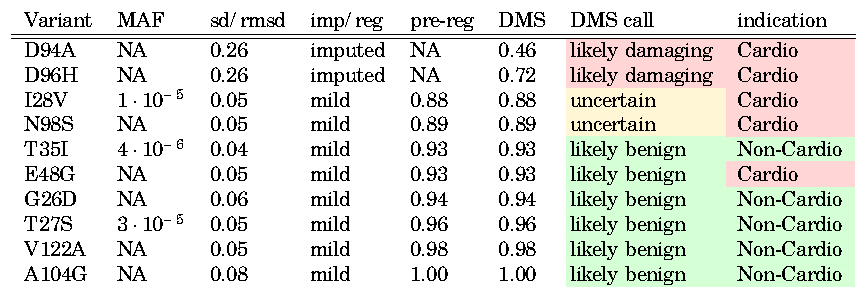
\includegraphics[width=\textwidth]{img/invitae.pdf}
	\label{tab:invitae}
\end{table}

% \begin{table}
% 	\centering
% 	\caption{}
% 	\begin{tabular}{l l l l l l l l}
% Variant & MAF & sd/rmsd & imp/reg & pre-reg & DMS & DMS call & indication \\ \hline\hline
% D94A & NA & 0.26 & imputed & NA & 0.46 & likely damaging & Cardio \\
% D96H & NA & 0.26 & imputed & NA & 0.72 & likely damaging & Cardio \\
% I28V & $1 \cdot 10^{-5}$ & 0.05 & mild & 0.88 & 0.88 & uncertain & Cardio \\
% N98S & NA & 0.05 & mild & 0.89 & 0.89 & uncertain & Cardio \\
% T35I & $4 \cdot 10^{-6}$ & 0.04 & mild & 0.93 & 0.93 & likely benign & Non-Cardio \\
% E48G & NA & 0.05 & mild & 0.93 & 0.93 & likely benign & Cardio \\
% G26D & NA & 0.06 & mild & 0.94 & 0.94 & likely benign & Non-Cardio \\
% T27S & $3 \cdot 10^{-5}$ & 0.05 & mild & 0.96 & 0.96 & likely benign & Non-Cardio \\
% V122A & NA & 0.05 & mild & 0.98 & 0.98 & likely benign & Non-Cardio \\
% A104G & NA & 0.08 & mild & 1.00 & 1.00 & likely benign & Non-Cardio
% 	\end{tabular}
% 	\label{tab:invitae}
% \end{table}



\section{Discussion}
\label{ch2discussion}

In total, this study has produced five maps with functional impacts for 15,998 possible missense variants. The functional maps generated for sumoylation pathway members UBE2I and SUMO1 and disease-implicated genes NCS1, CALM1/2/3 and TPK1 using the DMS framework were consistent with biochemical expectations while providing new hypotheses. DMS maps based on functional complementation were highly predictive of disease causing mutations, outperforming computational prediction methods such as PolyPhen-2 or PROVEAN.  The imputation method I employed allows me to generate complete functional maps while maintaining the reliability on par with the experimental results. 

Given the prospect of personalized and precision medicine, genome sequencing is expected to become increasingly common in everyday medical practice. Current estimates suggest that every human carries an average of 200-300 rare missense mutations that have never before been seen in the clinic~\cite{the_1000_genomes_project_consortium_global_2015}. This creates a need for fast, reliable interpretation of variant effects. Instead of generating clones and functionally testing variants of unknown significance after they are first observed, DMS technology offers to generate exhaustive maps of functional variation that enable interpretation immediately upon clinical presentation, even for rare and personal variation.

A key requirement for DMS mapping is an \textit{en masse} functional assay that can be applied at the scale of $10^4-10^5$ variant clones, such as complementation in yeast.  However, among $\sim 4000$ disease genes, examination of four systematic screens and curated literature suggests that only $\sim 5\%$ of human disease genes have a yeast complementation assay~\cite{hamza_complementation_2015,kachroo_systematic_2015,sun_extended_2016}. Complementation assays can also be carried out in human cells~\cite{wagenaar_resistance_2014}, and \textit{en masse} transfection is achievable at the required scale~\cite{blomen_gene_2015}. Based on only three large-scale CRISPR studies~\cite{hart_high-resolution_2015,blomen_gene_2015,wang_genetic_2014}, cellular growth phenotypes have already been observed in at least one cell line for 29\% of human disease genes.  Beyond complementation, sub-functional assays, e.g. of protein interaction, can not only reveal variation that impacts the specifically assayed sub-function but also folding/stability mutations that ablate overall function. In a recent study, approximately two thirds of disease-causing variants were found to impact at least one protein interaction~\cite{sahni_widespread_2015}. Although only a minority of human protein interactions have been mapped~\cite{rolland_proteome-scale_2014}, already 40\% of human genes have at least one interaction partner detectable by yeast two-hybrid assay in a recent screen~\cite{rolland_proteome-scale_2014}. Taking the union of available assays, one may estimate that 57\% of known disease-associated genes already have an assay potentially amenable to DMS. Emerging protein interaction data and CRISPR screens suggests that the proportion of DMS-accessible disease genes will continue to rise. 

\section{Methods}

\subsection{DMS-TileSeq}
The DMS-TileSeq experiment for \gene{SUMO1}, \gene{TPK1}, \gene{NCS1}, and \gene{CALM1} was performed by Song Sun and Marta Verby as described in chapter~\ref{ch:data1}. The downstream sequencing data analysis, scoring, imputation and regularization was performed by me as described in chapter~\ref{ch:data1}.

\subsection{DMS-BarSeq Y2H}
The DMS-BarSeq Y2H experiment was performed by Jennifer Knapp as described in chapter~\ref{ch:data1}, except for the following differences: (1) The \textit{en~masse} LR cloning of the UBE2I variant library was targeted into barcoded Y2H AD vectors; (2) Following KiloSeq and re-arraying, the library was pooled and transformed into haploid MATa yeast strains and mated with MAT$\alpha$ strains carrying SATB1-DB plasmids. Following diploid selection, the pool was grown for 48h in triplicates on Histidine-supplemented (permissive) and Histidine-deficient (selective) media, respectively. Plates were scraped and barcode loci amplified for BarSEQ.

Downstream sequencing data analysis and scoring was performed by me. Barcode counts were divided by the overall number of barcodes reads in each condition to obtain relative barcode frequency. Barcode frequencies in the -HIS condition were divided by frequencies in +HIS condition. Scores were then scaled to the null and WT controls, such that 0 corresponds to the average fitness of null controls and 1 to the average fitness of WT controls. Standard deviation based on technical replicates were regularized using the Baldi \& Long method as described in chapter~\ref{ch:data1}. The underlying code is part of a larger DMS analysis package provided on the attached storage media, and also available online\footnote{\url{http://dalai.mshri.on.ca/~jweile/projects/popcodePipeline/doc}}.

\subsection{UBE2I-SATB1 analysis}
I integrated the complementation and Y2H data and filtered out low-quality measurements ($\text{s.d.} > 0.3$). To find interface candidates, I then selected the set of variants for which (i) the complementation score was greater than 0.5, (ii) the Y2H score was less than 0.5, and (iii) the Y2H score is at least 0.5 units below the complementation score. I then mapped the resulting variants on the UBE2I crystal structure.

\subsection{UBE2I interface analysis}
Co-crystal structure data for UBE2I was obtained from the PDB (Entries: \texttt{3UIP}~\cite{gareau_determinants_2012}; \texttt{4W5V}~\cite{reiter_characterization_2016}; \texttt{3KYD}~\cite{olsen_active_2010}; \texttt{2UYZ}~\cite{knipscheer_noncovalent_2007}; \texttt{4Y1L}~\cite{alontaga_rwd_2015}). A custom script was developed to obtain solvent accessibility using \texttt{GETAREA}~\cite{fraczkiewicz_exact_1998} for monomers and complexes, allowing for the calculation of relative burial of interfacial residues. Complementation fitness distributions for each interaction's interfacial residues were tallied and tested for statistically significant differences using Wilcoxon tests. Distributions were plotted using the R package \texttt{beeswarm}~\cite{eklund_bee_2016}. The methods were implemented as part of a larger DMS analysis package provided on the attached storage media, and also available online\footnote{\url{http://dalai.mshri.on.ca/~jweile/projects/popcodePipeline/doc}}.


\subsection{Structure coloration} A custom script was developed to calculate median and maximum complementation fitness values for each residue and autogenerate coloration commands for OpenPyMol~\cite{schrodinger_pymol_2016}. The methods were implemented as part of a larger DMS analysis package provided on the attached storage media, and also available online\footnote{\url{http://dalai.mshri.on.ca/~jweile/projects/popcodePipeline/doc}}.

\subsection{Complementation spotting assays} Complementation spotting assays were performed by Jennifer Knapp as described in chapter~\ref{ch:data1}. Image data was processed using PlateOrganizer and integrated and compared to the high-throughput results using custom scripts.

\subsection{Hypercomplementing mutation analysis}
\paragraph{Hypercomplementation and reversion to yeast residues:} To examine whether changing amino acid residues into those residues naturally occur in yeast were more likely to show hyperactive complementation I compared these cases to changes into residues occurring in other species. The UBE2I amino acid sequence was aligned to that of its orthologues in \species{S.~cerevisiae}, \species{D.~discoideum} and \species{D.~melanogaster} using \texttt{CLUSTAL}~\cite{russell_clustal_2014}. A custom script was used to extract inter-species amino acid changes and lookup the corresponding complementation fitness values in the UBE2I map. Distributions were plotted using the R package \texttt{beeswarm}~\cite{eklund_bee_2016}. Wilcoxon tests revealed no significant differences between the distributions. The methods were implemented as part of a larger DMS analysis package provided on the attached storage media, and also available online\footnote{\url{http://dalai.mshri.on.ca/~jweile/projects/popcodePipeline/doc}}.

\paragraph{\textit{In vitro} sumoylation comparison} Images from \textit{in vitro} sumoylation assays performed for UBE2I variants by Bernier-Villamor~\etal~\cite{bernier-villamor_structural_2002} were scored by visual inspection while blinded to the underlying variant information. Scores were then represented as a heatmap and compared complementation scores from the UBE2I map. The methods were implemented as part of a larger DMS analysis package provided on the attached storage media, and also available online\footnote{\url{http://dalai.mshri.on.ca/~jweile/projects/popcodePipeline/doc}}.

\paragraph{Phylogenetic comparison of different models for hyperactive mutations}
The \texttt{phydms} software package~\cite{bloom_identification_2017} was used by Jesse Bloom to test three different models relating the effect of activity-enhancing mutations in SUMO1 and UBE2I to the actual evolutionary preference for that amino acid in a real biological context. Specifically, using the substitution models described in \cite{bloom_identification_2017}, three different ways of relating the evolutionary preference $\pi_{r,a}$ for amino-acid a at site $r$ to the fitness score $f_{r,a}$ for a given mutation were tested. 

In the first model, $$\pi_{r,a} = f_{r,a}.$$ 

In the second model, $$\pi_{r,a} = \min(f_{r,a}, f_{r,\text{wt}}),$$ where $f_{r,\text{wt}}$ is the fitness score for the wildtype amino-acid at site $r$. 

Finally, in the third model, $$\pi_{r,a} = \begin{cases} f_{r,a} &  \text{if}~ f_{r,a} \le f_{r,\text{wt}} \\ \frac{1}{f_{r,a}} & \text{otherwise} \end{cases}. $$ 

Each of these models were fit to the set of Ensembl homologues with at least 75\% sequence identity to the human protein. 

\subsection{Transformation of maps for human phenotypes}
Having established the third substitution model to provide the best fit for evolutionary preference (see above), I applied the corresponding transformation function underlying the model to the complementation data for each tested gene and repeated the imputation and regularization steps described in the previous chapter on the transformed data.

\subsection{Intragenic epistasis analysis} Genetic interactions were determined based on a previously described multiplicative model~\cite{phillips_language_1998,onge_systematic_2007}, that expects double mutant fitness to conform to the product of single mutant fitness effects in the absence of interaction between the two. Under this model, the strength of genetic interaction is defined as $$\varepsilon_{ij} = f_i \cdot f_j - f_{ij},$$ where $f_i$ and $f_j$ represent single mutant fitness and $f_{ij}$ represents double mutant fitness scores. To test for deviation from this model, all cases where double mutant and both corresponding single mutants were known in the data were extracted. The standard deviation for the expected double mutant fitness $f_i \cdot f_j$ was estimated using
$$ \mathbb{V}(XY) = \mathbb{E}(X^2Y^2)-(\mathbb{E}(XY))^2=\mathbb{V}(X)\mathbb{V}(Y) + \mathbb{V}(X)(\mathbb{E}(Y))^2+\mathbb{V}(Y)(\mathbb{E}(X))^2 $$ 
%$$ \bar{\sigma}_{i,j} = \sqrt{\sigma_i^2 \cdot \sigma_j^2 + \sigma_i^2 \cdot \mu_j^2 + \sigma_j^2 \cdot \mu_i^2},$$ 
%where $\sigma_i , \sigma_j$ are the standard deviations and $\mu_i , \mu_j$ are the means of the single mutant fitness measurements.
Using these estimates, Student t-tests were performed between the measured and expected double mutant fitnesses and corrected for multiple hypothesis testing using the  Benjamini-Hochberg~\cite{benjamini_controlling_1995} method at a 5\% FDR threshold.

To detect potential direct compensatory relationships, the genetic interactions were compared with physical distance in the protein's 3D structure. The Euclidean distance between the C$_\alpha$ atoms in of each pair of residues was calculated using a custom script using structural data from the PDB (\texttt{3UIP}~\cite{gareau_determinants_2012}).
The methods were implemented as part of a larger DMS analysis package provided on the attached storage media, and also available online\footnote{\url{http://dalai.mshri.on.ca/~jweile/projects/popcodePipeline/doc}}.



\subsection{Structural analysis of disease gene maps}
Co-crystal and NMR structure data for SUMO1, TPK1, NCS1 and CALM1 was obtained from the PDB (Entries: \texttt{2G4D}~\cite{xu_crystal_2006}; \texttt{2IO2}~\cite{reverter_structural_2006}; \texttt{3KYD}~\cite{olsen_active_2010}; \texttt{3UIP}~\cite{gareau_determinants_2012}; \texttt{2ASQ}~\cite{song_small_2005}; \texttt{4WJO}~\cite{cappadocia_structural_2015-1}; \texttt{4WJQ}~\cite{cappadocia_structural_2015-1}; \texttt{1WYW}~\cite{baba_crystal_2005}; 
\texttt{2L2E}~(Ames \etal\ unpublished); \texttt{4GUK}~(Chengpeng \etal\ unpublished); \texttt{5AFP}~\cite{pandalaneni_neuronal_2015}; 
\texttt{3G43}~\cite{fallon_crystal_2009}; \texttt{4DJC}~\cite{sarhan_crystallographic_2012}; 
\texttt{3S4Y}~\cite{timm_crystal_2001}; ). Structures were colorized using the same method described above for UBE2I and analyzed using OpenPyMol~\cite{schrodinger_pymol_2016}.

%NCS1: 2L2E myristoylated NCS1 (pombe) Ames et al unpublished
%  -> 4GUK (plain) Chengpeng, F., Elias, L. unpublished
%  -> 5AFP (rhodopsin kinase) (rat) Pandalaneni et al http://dx.doi.org/10.1074/jbc.M114.627059
%Calmodulin: 3G43 (ca channel fragm.) Fallon et al. http://www.pnas.org/content/106/13/5135
%  -> 4DJC (na channel fragm.) sarhan et al http://dx.doi.org/10.1073/pnas.1114748109
%TPK1: 3S4Y timm_crystal_2001
%SUMO1:
% -> 2G4D (SENP1) Xu et al, http://dx.doi.org/10.1042/BJ20060526
% -> 2IO2(SENP2) Reverter et al, http://dx.doi.org/10.1038/nsmb1168
% -> 3KYD (E1) olsen_active_2010
% -> 3uip
% -> 2ASQ (PIAS2) Song et al http://dx.doi.org/10.1074/jbc.M507059200
% -> 4WJO (PML) Cappadocia http://dx.doi.org/10.1016/j.str.2014.10.015
% -> 4WJQ (DAXX) Cappadocia (same as PML)
% -> 1WYW (TDG) Baba et al http://dx.doi.org/10.1038/nature03634


\subsection{Disease variant analysis}
Missense variant tables for \gene{UBE2I}, \gene{SUMO1}, \gene{TPK1}, \gene{NCS1}, \gene{CALM1}, \gene{CALM2} and \gene{CALM3} were integrated ClinVar, COSMIC, and GnomAD and compared with complementation scores. To calculate diploid scores for TPK1, phased variant call files (VCF) for the TPK1 gene obtained from the 1000 genomes project database to identify homozygous, heterozygous and compound heterozygous cases for all present variants using a custom script. For each case, the diploid score was calculated as $s_\text{diploid} = \max(s_1,s_2)$, where $s_1$ and $s_2$ are the variant scores for the paternal and maternal allele. The methods were implemented as part of a larger DMS analysis package provided on the attached storage media, and also available online\footnote{\url{http://dalai.mshri.on.ca/~jweile/projects/popcodePipeline/doc}}.